\PassOptionsToPackage{unicode}{hyperref}
\PassOptionsToPackage{hyphens}{url}
\documentclass[]{article}

% ============================================================
%  CONFIGURACIÓN DE PÁGINA Y MÁRGENES
% ============================================================
\usepackage[margin=2.5cm]{geometry}
\usepackage{setspace}
\setstretch{1.1}
\setlength{\parskip}{4pt}
\setlength{\parindent}{0pt}

% ============================================================
%  FONDO (BACKGROUND)
% ============================================================
\usepackage[pages=all]{background}
\backgroundsetup{
  scale=1,
  color=black,
  opacity=1,
  angle=0,
  contents={%
    
\includegraphics[width=\paperwidth,height=\paperheight]{./media/fondo.png}%
  }
}

% ============================================================
%  PAQUETES MATEMÁTICOS BASE (Cargar antes de unicode-math)
% ============================================================
\usepackage{amsmath,amssymb}

% ============================================================
%  IDIOMA, TIPOGRAFÍA Y FUENTES (Compatible con pdfLaTeX y XeLaTeX/LuaLaTeX)
% ============================================================
\usepackage{iftex}
\ifPDFTeX
  \usepackage[T1]{fontenc}
  \usepackage[utf8]{inputenc}
  \usepackage{textcomp}
\else % XeLaTeX o LuaTeX
  \usepackage{unicode-math}
  \defaultfontfeatures{Scale=MatchLowercase}
  \defaultfontfeatures[\rmfamily]{Ligatures=TeX,Scale=1}
\fi
\usepackage{lmodern}
\usepackage[spanish,es-tabla]{babel}

% ============================================================
%  PAQUETES GRÁFICOS Y DIAGRAMAS
% ============================================================
\usepackage{graphicx}
\usepackage{xcolor}
\usepackage{float}
\usepackage{pgfplots}
\pgfplotsset{compat=1.16}
\usetikzlibrary{babel}

% ============================================================
%  TABLAS Y LISTAS
% ============================================================
\usepackage{tabularx}
\usepackage{longtable,booktabs,array}
\usepackage{calc}
\usepackage{enumitem}
\usepackage{caption}
\captionsetup{font=small,labelfont=bf}

\newcounter{none} % Contador para tablas sin numerar

\usepackage{etoolbox}
\makeatletter
\patchcmd\longtable{\par}{\if@noskipsec\mbox{}\fi\par}{}{}
\makeatother

\IfFileExists{footnotehyper.sty}{\usepackage{footnotehyper}}{\usepackage{footnote}}
\makesavenoteenv{longtable}

% ============================================================
%  LISTINGS (CÓDIGO FUENTE PYTHON CON ACENTOS)
% ============================================================
\usepackage{listings}
\lstset{
  language=Python,
  basicstyle=\ttfamily\footnotesize,
  keywordstyle=\color{blue!60!black},
  commentstyle=\color{green!40!black},
  stringstyle=\color{red!50!black},
  showstringspaces=false,
  breaklines=true,
  frame=single,
  numbers=left,
  numberstyle=\tiny\color{gray},
  xleftmargin=1.5em,
  framexleftmargin=1.5em,
  literate={á}{{\'a}}1 {é}{{\'e}}1 {í}{{\'i}}1 {ó}{{\'o}}1 {ú}{{\'u}}1
           {Á}{{\'A}}1 {É}{{\'E}}1 {Í}{{\'I}}1 {Ó}{{\'O}}1 {Ú}{{\'U}}1
           {ñ}{{\~n}}1 {Ñ}{{\~N}}1
}

% ============================================================
%  FORMATO ADICIONAL Y PANDOC
% ============================================================
\setcounter{secnumdepth}{-\maxdimen} % Elimina numeración si es necesario

\IfFileExists{upquote.sty}{\usepackage{upquote}}{}
\IfFileExists{microtype.sty}{%
  \usepackage[]{microtype}
  \UseMicrotypeSet[protrusion]{basicmath}
}{}

\makeatletter
\@ifundefined{KOMAClassName}{%
  \IfFileExists{parskip.sty}{%
    \usepackage{parskip}
  }{%
    \setlength{\parindent}{0pt}
    \setlength{\parskip}{6pt plus 2pt minus 1pt}}
}{%
  \KOMAoptions{parskip=half}}
\makeatother

\makeatletter
\newsavebox\pandoc@box
\newcommand*\pandocbounded[1]{%
  \sbox\pandoc@box{#1}%
  \Gscale@div\@tempa{\textheight}{\dimexpr\ht\pandoc@box+\dp\pandoc@box\relax}%
  \Gscale@div\@tempb{\linewidth}{\wd\pandoc@box}%
  \ifdim\@tempb\p@<\@tempa\p@\let\@tempa\@tempb\fi%
  \ifdim\@tempa\p@<\p@\scalebox{\@tempa}{\usebox\pandoc@box}%
  \else\usebox{\pandoc@box}%
  \fi%
}
\def\fps@figure{htbp}
\makeatother

\setlength{\emergencystretch}{3em}
\providecommand{\tightlist}{%
  \setlength{\itemsep}{0pt}\setlength{\parskip}{0pt}}

% ============================================================
%  ENLACES Y MARCADORES
% ============================================================
\usepackage{bookmark}
\IfFileExists{xurl.sty}{\usepackage{xurl}}{}
\urlstyle{same}
\hypersetup{
  hidelinks,
  pdfcreator={LaTeX via pandoc}}

\author{}
\date{}

\begin{document}

INGENIERÍA EN CIENCIA DE DATOS E INTELIGENCIA ARTIFICIAL

Portfolio digital de la materia: Fundamentos de Machine learning

Equipo: Alt F4

Grado: Tercero Grupo: R

\section{Indice de las investigaciones}\label{indice}

\hyperref[investigaciuxf3n-de-outliers-cuartiles-puntuaciuxf3n-z-estandarizar-y-normalizar]{INVESTIGACIÓN
DE OUTLIERS ,CUARTILES, PUNTUACIÓN Z, ESTANDARIZAR Y NORMALIZAR
\hyperref[investigaciuxf3n-de-outliers-cuartiles-puntuaciuxf3n-z-estandarizar-y-normalizar]{4}}

\hyperref[outliers]{OUTLIERS \hyperref[outliers]{5}}

\hyperref[cuartiles]{CUARTILES \hyperref[cuartiles]{6}}

\hyperref[puntuaciuxf3n-z]{PUNTUACIÓN Z \hyperref[puntuaciuxf3n-z]{7}}

\hyperref[estandarizar]{ESTANDARIZAR \hyperref[estandarizar]{8}}

\hyperref[normalizar]{NORMALIZAR \hyperref[normalizar]{10}}

\hyperref[referencias]{REFERENCIAS: \hyperref[referencias]{11}}

\hyperref[investigaciuxf3n-knn-one-hot-encoding-y-label-encoding]{INVESTIGACIÓN
KNN, ONE-HOT ENCODING Y LABEL ENCODING
\hyperref[investigaciuxf3n-knn-one-hot-encoding-y-label-encoding]{12}}

\hyperref[introducciuxf3n]{1. Introducción
\hyperref[introducciuxf3n]{13}}

\hyperref[knn-k-nearest-neighbors]{2. KNN (K-Nearest Neighbors)
\hyperref[knn-k-nearest-neighbors]{13}}

\hyperref[one-hot-encoding]{3. One-Hot Encoding
\hyperref[one-hot-encoding]{14}}

\hyperref[label-encoding]{4. Label Encoding
\hyperref[label-encoding]{14}}

\hyperref[diferencias-entre-las-tuxe9cnicas]{5. Diferencias entre las
técnicas \hyperref[diferencias-entre-las-tuxe9cnicas]{15}}

\hyperref[cuxf3mo-realizarlo-en-excel-paso-a-paso]{6. Cómo realizarlo en
Excel paso a paso
\hyperref[cuxf3mo-realizarlo-en-excel-paso-a-paso]{15}}

\hyperref[preparar-los-datos]{6.1 Preparar los datos
\hyperref[preparar-los-datos]{15}}

\hyperref[one-hot-encoding-en-excel]{6.2 One-Hot Encoding en Excel
\hyperref[one-hot-encoding-en-excel]{16}}

\hyperref[label-encoding-en-excel]{6.3 Label Encoding en Excel
\hyperref[label-encoding-en-excel]{16}}

\hyperref[knn-en-excel-paso-a-paso]{6.4 KNN en Excel paso a paso
\hyperref[knn-en-excel-paso-a-paso]{17}}

\hyperref[programaciuxf3n-en-python]{7. Programación en Python
\hyperref[programaciuxf3n-en-python]{18}}

\hyperref[instalaciuxf3n]{7.1 Instalación \hyperref[instalaciuxf3n]{18}}

\hyperref[one-hot-encoding-con-python]{7.2 One-Hot Encoding con Python
\hyperref[one-hot-encoding-con-python]{18}}

\hyperref[label-encoding-con-python]{7.3 Label Encoding con Python
\hyperref[label-encoding-con-python]{19}}

\hyperref[knn-completo-con-one-hot-encoding]{7.4 KNN completo con
One-Hot Encoding \hyperref[knn-completo-con-one-hot-encoding]{19}}

\hyperref[ejemplo-de-predicciuxf3n]{8. Ejemplo de predicción
\hyperref[ejemplo-de-predicciuxf3n]{20}}

\hyperref[quuxe9-tuxe9cnica-conviene-utilizar]{9. ¿Qué técnica conviene
utilizar? \hyperref[quuxe9-tuxe9cnica-conviene-utilizar]{20}}

\hyperref[conclusiuxf3n]{10. Conclusión \hyperref[conclusiuxf3n]{21}}

\hyperref[referencias-1]{11. Referencias \hyperref[referencias-1]{21}}

\hyperref[data-leak]{DATA LEAK \hyperref[data-leak]{22}}

\hyperref[referencias-2]{Referencias: \hyperref[referencias-2]{26}}

\hyperref[errores-mae-mse-rmse-mape]{Errores Mae, Mse, Rmse, Mape
\hyperref[errores-mae-mse-rmse-mape]{27}}

\hyperref[referencias-3]{Referencias: \hyperref[referencias-3]{41}}

\hyperref[inv1]{Matriz de confusion}

\section{Indice de las documentaciones}\label{indice-doc}

\hyperref[intrdoc]{Documentacion de los codigos en clase}

\hyperref[doc1]{Documentación del código de regresión mulltivariada}

\hyperref[doc2]{Documentación del codigo de regresión logistica}

\newpage
\section{INVESTIGACIÓN DE OUTLIERS ,CUARTILES, PUNTUACIÓN Z,
ESTANDARIZAR Y
NORMALIZAR}\label{investigaciuxf3n-de-outliers-cuartiles-puntuaciuxf3n-z-estandarizar-y-normalizar}

Carrera: Ingeniería en ciencia de datos he inteligencia artificial

Equipo: Alt F4

\textbf{\hfill\break
}

\subsection{OUTLIERS}\label{outliers}

\textbf{¿Qué son los valores atípicos (outliers)?}

En estadística, los valores atípicos, también llamados~observaciones
atípicas u outliers, Es decir, un valor atípico es un valor anormal y
que es extremadamente diferente al resto de valores de la muestra. No es
necesariamente un error pero distorsiona la media y el análisis y hay
que decir si se elimina o se conserva.

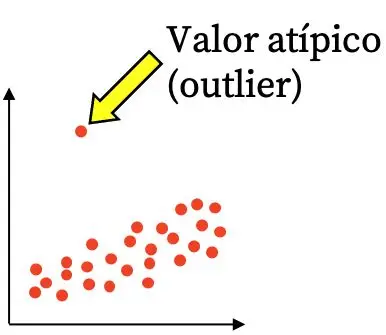
\includegraphics[width=2.32558in,height=2.01832in]{./media/image1.png}

En \textbf{Excel}, una forma confiable de detectar outliers (valores
atípicos) es usando el método del Rango Intercuartílico (IQR).

\textbf{Método IQR en Excel}

El IQR se calcula así: \(\text{IQR} = Q3 - Q1\)

Donde:

\begin{itemize}
\item
  \textbf{Q1}~= Primer cuartil (25\% de los datos)
\item
  \textbf{Q3}~= Tercer cuartil (75\% de los datos)
\end{itemize}

Un valor es~outlier~si:

\begin{itemize}
\item
  \textbf{Menor que:}~\(Q1 - 1.5 \times IQR\)
\item
  \textbf{Mayor que:}~\(Q3 + 1.5 \times IQR\)
\end{itemize}

\subsection{CUARTILES}\label{cuartiles}

En la página anterior se mencionaron los cuartiles pero ¿Qué son los
cuartiles?

En estadística, los cuartiles son los tres valores que dividen a un
conjunto de datos ordenados en cuatro partes iguales.~Por lo tanto, el
primer, segundo y tercer cuartil representan respectivamente el 25\%,
50\% y 75\% del conjunto de datos estadísticos.

Los cuartiles se representan mediante una Q mayúscula y el subíndice del
cuartil, de manera que el primer cuartil es Q\textsubscript{1}, el
segundo cuartil es Q\textsubscript{2}, y el tercer cuartil es
Q\textsubscript{3}.

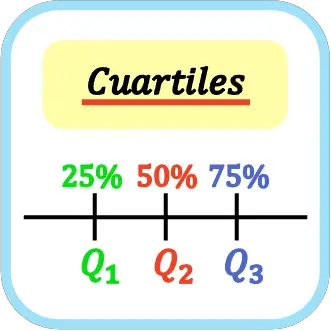
\includegraphics[width=3.19767in,height=3.19767in]{./media/image2.png}

\subsection{PUNTUACIÓN Z}\label{puntuaciuxf3n-z}

\textbf{¿Qué es la puntuación Z?}

La~\textbf{puntuación Z}, o \textbf{puntaje Z}, es una puntuación
estadística que indica a cuántas desviaciones estándar de la media se
encuentra un valor. Para calcular una puntuación Z de un valor se debe
restar la media a dicho valor y luego dividir por la desviación estándar
de la muestra de datos.

Por ejemplo, si un valor se encuentra dos desviaciones estándar por
debajo de la media aritmética del conjunto de datos, la puntuación Z de
ese valor es igual a -2.

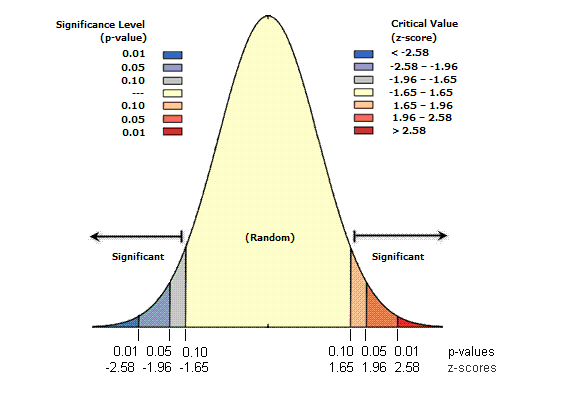
\includegraphics[width=3.79969in,height=2.63978in]{./media/image3.png}

En Excel, este cálculo puede realizarse de diferentes maneras. Una forma
consiste en hacerlo paso a paso: primero se obtiene la media mediante la
función PROMEDIO, después la desviación estándar con DESVEST.P si se
trabaja con toda la población o con DESVEST.M si se trata de una
muestra, y finalmente se aplica la fórmula \((A2 - \mu)/\sigma\)para
cada valor de la serie.

Otra alternativa es emplear una fórmula directa que combine todos los
cálculos en una sola expresión, evitando el uso de celdas auxiliares.
Por ejemplo, para una población se utiliza: =(A2 -
PROMEDIO(\$A\$2:\$A\$11)) / DESVEST.P(\$A\$2:\$A\$11) y para una muestra
se reemplaza por DESVEST.M.

Excel también ofrece la función integrada ESTANDARIZAR, que simplifica
el procedimiento al calcular automáticamente el Z-score de cada dato a
partir de la media y la desviación estándar del rango seleccionado.

Es fundamental tener presente que un Z-score positivo indica que el
valor se encuentra por encima de la media, mientras que un Z-score
negativo señala que está por debajo. Asimismo, la elección entre
DESVEST.P y DESVEST.M depende de si se dispone de toda la población o
únicamente de una muestra.

\subsection{ESTANDARIZAR}\label{estandarizar}

La estandarización es una técnica estadística que se utiliza para
transformar los datos en un formato común, lo que permite una
comparación y un análisis más sencillos. Este proceso implica ajustar
los valores de un conjunto de datos para que tengan una media de cero y
una desviación estándar de uno.

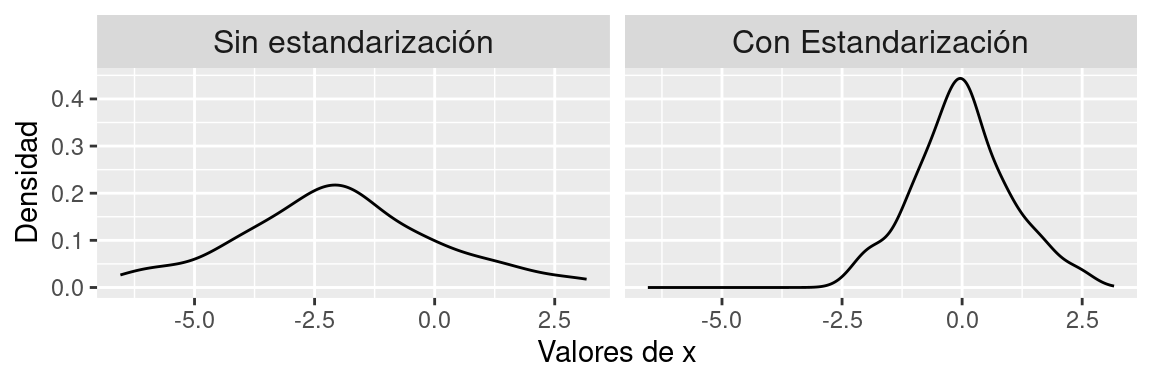
\includegraphics[width=6.00004in,height=2.00001in]{./media/image4.png}

\textbf{¿Cómo aplicar la estandarización en Excel?}

\begin{enumerate}
\def\labelenumi{\arabic{enumi}.}
\item
  Coloca los datos que deseas estandarizar en una columna, por ejemplo,
  de A2:A11.
\item
  Calcula la media de los datos con:\\
  =PROMEDIO(A2:A11)
\item
  Calcula la desviación estándar:

  \begin{itemize}
  \item
    Para una población: =DESVEST.P(A2:A11)
  \item
    Para una muestra: =DESVEST.M(A2:A11)
  \end{itemize}
\item
  En una nueva columna, aplica la fórmula de puntuación Z:\\
  =(A2-PROMEDIO(\$A\$2:\$A\$11))/DESVEST.M(\$A\$2:\$A\$11)
\item
  Presiona Enter y arrastra la fórmula hacia abajo para obtener la
  estandarización de todos los datos.
\end{enumerate}

También puedes utilizar directamente la función ``ESTANDARIZAR'' de
Excel:

=ESTANDARIZAR(A2,PROMEDIO(\$A\$2:\$A\$11),DESVEST.M(\$A\$2:\$A\$11))

De esta manera, cada dato se transforma a su valor estandarizado (Z),
permitiendo comparar los datos independientemente de su escala original.

\subsection{NORMALIZAR}\label{normalizar}

En el análisis de datos, la~\textbf{normalización estadística}~es una
técnica fundamental que permite transformar diferentes variables para
que puedan ser comparadas y utilizadas de manera uniforme. La
normalización es un proceso que ajusta los valores de los datos a una
escala común, sin distorsionar las diferencias en los rangos de valores.

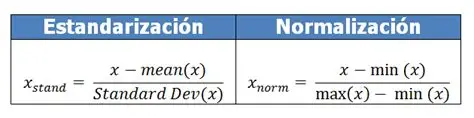
\includegraphics[width=6.5in,height=1.61806in]{./media/image5.png}

\textbf{¿Cómo aplicar la normalización en Excel?}

\begin{enumerate}
\def\labelenumi{\arabic{enumi}.}
\item
  Coloca los datos en una columna, por ejemplo, \textbf{A2:A11}.
\item
  En una nueva columna, escribe la fórmula:
\end{enumerate}

=(A2-MIN(\$A\$2:\$A\$11))/(MAX(\$A\$2:\$A\$11)-MIN(\$A\$2:\$A\$11))

\begin{enumerate}
\def\labelenumi{\arabic{enumi}.}
\setcounter{enumi}{2}
\item
  Presiona \textbf{Enter}.
\item
  Arrastra la fórmula hacia abajo para aplicarla a todos los datos.
\end{enumerate}

Con esto:

\begin{itemize}
\item
  El \textbf{valor mínimo} se convierte en \textbf{0}.
\item
  El \textbf{valor máximo} se convierte en \textbf{1}.
\item
  Los demás valores quedan entre \textbf{0 y 1}, manteniendo la
  proporción entre ellos.
\end{itemize}

\subsection{REFERENCIAS:}\label{referencias}

\href{https://www.probabilidadyestadistica.net/valores-atipicos-outliers/}{$\triangleright$
Valores atípicos (outliers): qué son, ejemplos, calculadora,...}

\href{https://www.probabilidadyestadistica.net/cuartiles/}{$\triangleright$ Cuartiles:
qué son, fórmula, ejemplos, calculadora...}

\href{https://www.probabilidadyestadistica.net/puntuacion-z/}{$\triangleright$
Puntuación Z (estadística)}

\href{https://estudyando.com/normalizacion-estadistica-conceptos-metodos-y-aplicaciones/}{Normalización
Estadística: Conceptos, Métodos y Aplicaciones \textbar{} Estudyando}

\href{https://es.statisticseasily.com/glosario/\%C2\%BFQu\%C3\%A9-es-la-estandarizaci\%C3\%B3n-de-datos\%3F/}{Qué
es: Estandarizar - Entender la estandarización de datos}

\section{INVESTIGACIÓN KNN, ONE-HOT ENCODING Y LABEL
ENCODING}\label{investigaciuxf3n-knn-one-hot-encoding-y-label-encoding}

Carrera: Ingeniería en ciencia de datos he inteligencia artificial

Equipo: Alt F4

\subsection{1. Introducción}\label{introducciuxf3n}

En aprendizaje automático es común trabajar con datos que contienen
categorías, como sexo, ciudad, tipo de producto o sistema operativo.
Muchos algoritmos necesitan que las variables estén representadas
numéricamente. El KNN (K-Nearest Neighbors) es un algoritmo de
aprendizaje supervisado que clasifica un dato según las clases de sus
vecinos más cercanos. Para utilizar variables categóricas con algoritmos
como KNN, es necesario aplicar técnicas de codificación como One-Hot
Encoding o Label Encoding.

\subsection{2. KNN (K-Nearest Neighbors)}\label{knn-k-nearest-neighbors}

KNN significa K-Nearest Neighbors o K vecinos más cercanos. Es un
algoritmo de aprendizaje supervisado utilizado principalmente para
clasificación y también para regresión. Para clasificar una observación,
calcula su distancia respecto de ejemplos conocidos, selecciona los K
vecinos más cercanos y, en clasificación, asigna la clase que tenga
mayor representación entre ellos.

La distancia euclidiana entre dos puntos puede calcularse como:

\[d = \sqrt{(x_1-x_2)^2 + (y_1-y_2)^2 + \ldots{} + (x_n-x_n')^2}\]

El valor K debe elegirse con cuidado. Un K pequeño puede hacer al modelo
sensible al ruido, mientras que un K demasiado grande puede suavizar
demasiado las diferencias entre clases. En scikit-learn,
KNeighborsClassifier implementa la votación de los K vecinos más
cercanos.

\subsection{3. One-Hot Encoding}\label{one-hot-encoding}

One-Hot Encoding convierte una variable categórica en varias columnas
binarias. Se crea una columna para cada categoría y se coloca 1 cuando
la observación pertenece a esa categoría y 0 cuando no pertenece. Es
especialmente útil cuando las categorías no tienen un orden natural,
porque evita que el modelo interprete que una categoría es numéricamente
mayor o menor que otra.

Ejemplo:

{\def\LTcaptype{none} % do not increment counter
\begin{longtable}[]{@{}
  >{\raggedright\arraybackslash}p{(\linewidth - 6\tabcolsep) * \real{0.2315}}
  >{\raggedright\arraybackslash}p{(\linewidth - 6\tabcolsep) * \real{0.2315}}
  >{\raggedright\arraybackslash}p{(\linewidth - 6\tabcolsep) * \real{0.2315}}
  >{\raggedright\arraybackslash}p{(\linewidth - 6\tabcolsep) * \real{0.2315}}@{}}
\toprule\noalign{}
\begin{minipage}[b]{\linewidth}\raggedright
Color
\end{minipage} & \begin{minipage}[b]{\linewidth}\raggedright
Rojo
\end{minipage} & \begin{minipage}[b]{\linewidth}\raggedright
Azul
\end{minipage} & \begin{minipage}[b]{\linewidth}\raggedright
Verde
\end{minipage} \\
\midrule\noalign{}
\endhead
\bottomrule\noalign{}
\endlastfoot
Rojo & 1 & 0 & 0 \\
Azul & 0 & 1 & 0 \\
Verde & 0 & 0 & 1 \\
\end{longtable}
}

\subsection{4. Label Encoding}\label{label-encoding}

Label Encoding asigna un número entero a cada categoría. Por ejemplo,
una variable Color podría codificarse como Azul=0, Rojo=1 y Verde=2. Es
sencillo y reduce el número de columnas, pero hay que tener cuidado:
para variables nominales sin orden, algunos algoritmos pueden
interpretar artificialmente que 2 es mayor que 1 y que 1 es mayor que 0.

{\def\LTcaptype{none} % do not increment counter
\begin{longtable}[]{@{}
  >{\raggedright\arraybackslash}p{(\linewidth - 2\tabcolsep) * \real{0.4620}}
  >{\raggedright\arraybackslash}p{(\linewidth - 2\tabcolsep) * \real{0.4620}}@{}}
\toprule\noalign{}
\begin{minipage}[b]{\linewidth}\raggedright
Color
\end{minipage} & \begin{minipage}[b]{\linewidth}\raggedright
Código
\end{minipage} \\
\midrule\noalign{}
\endhead
\bottomrule\noalign{}
\endlastfoot
Azul & 0 \\
Rojo & 1 \\
Verde & 2 \\
\end{longtable}
}

\subsection{5. Diferencias entre las
técnicas}\label{diferencias-entre-las-tuxe9cnicas}

{\def\LTcaptype{none} % do not increment counter
\begin{longtable}[]{@{}
  >{\raggedright\arraybackslash}p{(\linewidth - 6\tabcolsep) * \real{0.2315}}
  >{\raggedright\arraybackslash}p{(\linewidth - 6\tabcolsep) * \real{0.2315}}
  >{\raggedright\arraybackslash}p{(\linewidth - 6\tabcolsep) * \real{0.2315}}
  >{\raggedright\arraybackslash}p{(\linewidth - 6\tabcolsep) * \real{0.2315}}@{}}
\toprule\noalign{}
\begin{minipage}[b]{\linewidth}\raggedright
Técnica
\end{minipage} & \begin{minipage}[b]{\linewidth}\raggedright
Resultado
\end{minipage} & \begin{minipage}[b]{\linewidth}\raggedright
Ventaja
\end{minipage} & \begin{minipage}[b]{\linewidth}\raggedright
Precaución
\end{minipage} \\
\midrule\noalign{}
\endhead
\bottomrule\noalign{}
\endlastfoot
KNN & Clasifica/regresa usando vecinos & Simple e intuitivo & La
distancia y la escala de las variables importan \\
One-Hot Encoding & Una columna 0/1 por categoría & No impone orden entre
categorías & Puede aumentar mucho el número de columnas \\
Label Encoding & Un número por categoría & Simple y compacto & Puede
introducir un orden artificial en variables nominales \\
\end{longtable}
}

\subsection{6. Cómo realizarlo en Excel paso a
paso}\label{cuxf3mo-realizarlo-en-excel-paso-a-paso}

\subsubsection{6.1 Preparar los datos}\label{preparar-los-datos}

Crea una tabla con datos de ejemplo. Por ejemplo: Edad, Color y Clase.
Puedes usar Edad como variable numérica, Color como variable categórica
y Clase como resultado.

{\def\LTcaptype{none} % do not increment counter
\begin{longtable}[]{@{}
  >{\raggedright\arraybackslash}p{(\linewidth - 6\tabcolsep) * \real{0.2315}}
  >{\raggedright\arraybackslash}p{(\linewidth - 6\tabcolsep) * \real{0.2315}}
  >{\raggedright\arraybackslash}p{(\linewidth - 6\tabcolsep) * \real{0.2315}}
  >{\raggedright\arraybackslash}p{(\linewidth - 6\tabcolsep) * \real{0.2315}}@{}}
\toprule\noalign{}
\begin{minipage}[b]{\linewidth}\raggedright
Edad
\end{minipage} & \begin{minipage}[b]{\linewidth}\raggedright
Color
\end{minipage} & \begin{minipage}[b]{\linewidth}\raggedright
Clase
\end{minipage} & \begin{minipage}[b]{\linewidth}\raggedright
Fila
\end{minipage} \\
\midrule\noalign{}
\endhead
\bottomrule\noalign{}
\endlastfoot
20 & Rojo & A & 1 \\
22 & Azul & B & 2 \\
21 & Rojo & A & 3 \\
25 & Verde & B & 4 \\
24 & Azul & B & 5 \\
19 & Rojo & A & 6 \\
\end{longtable}
}

\subsubsection{6.2 One-Hot Encoding en
Excel}\label{one-hot-encoding-en-excel}

1. Coloca las categorías como encabezados de nuevas columnas. Por
ejemplo: Color\_Rojo, Color\_Azul y Color\_Verde.

2. En la primera fila de datos, escribe una fórmula para comprobar si el
valor coincide con el encabezado.

3. Para Color\_Rojo, si el color está en B2, puedes usar:
=SI(\$B2="Rojo";1;0)

4. Para Color\_Azul: =SI(\$B2="Azul";1;0)

5. Para Color\_Verde: =SI(\$B2="Verde";1;0)

6. Arrastra las fórmulas hacia abajo para todas las filas.

7. El resultado será una matriz de 0 y 1. Esta es la representación
One-Hot.

\subsubsection{6.3 Label Encoding en
Excel}\label{label-encoding-en-excel}

Una forma sencilla es crear una tabla de equivalencias. Por ejemplo:
Azul=0, Rojo=1 y Verde=2.

1. En otra zona de la hoja crea una tabla con las categorías y sus
códigos.

2. Si tienes Excel moderno, usa BUSCARX para recuperar el código
correspondiente.

3. Ejemplo: =BUSCARX(B2;\$H\$2:\$H\$4;\$I\$2:\$I\$4)

4. Copia la fórmula hacia abajo.

5. Revisa que todas las categorías hayan recibido un código.

\subsubsection{6.4 KNN en Excel paso a
paso}\label{knn-en-excel-paso-a-paso}

1. Convierte primero las variables categóricas a números mediante
One-Hot Encoding o Label Encoding, según el caso.

2. Si las variables numéricas tienen escalas muy diferentes, considera
normalizarlas o estandarizarlas.

3. Define el nuevo punto que deseas clasificar.

4. Calcula la distancia euclidiana entre el nuevo punto y cada
observación conocida. Por ejemplo, para dos variables:
=RAIZ((A2-\$J\$2)\^{}2+(B2-\$K\$2)\^{}2)

5. Copia la fórmula para todas las observaciones.

6. Ordena las distancias de menor a mayor.

7. Selecciona los K vecinos más cercanos. Por ejemplo, si K=3, toma las
tres distancias menores.

8. Observa las clases de esos vecinos y asigna al nuevo punto la clase
que aparezca con mayor frecuencia.

\subsection{7. Programación en Python}\label{programaciuxf3n-en-python}

En Python se pueden utilizar pandas y scikit-learn. OneHotEncoder está
disponible en sklearn.preprocessing y KNeighborsClassifier en
sklearn.neighbors.

\subsubsection{7.1 Instalación}\label{instalaciuxf3n}

En la terminal o en Google Colab:

pip install pandas scikit-learn

\subsubsection{7.2 One-Hot Encoding con
Python}\label{one-hot-encoding-con-python}

import pandas as pd\\
from sklearn.preprocessing import OneHotEncoder\\
\strut \\
df = pd.DataFrame(\{\\
"Edad": {[}20, 22, 21, 25, 24, 19{]},\\
"Color": {[}"Rojo", "Azul", "Rojo", "Verde", "Azul", "Rojo"{]}\\
\})\\
\strut \\
encoder = OneHotEncoder(sparse\_output=False)\\
resultado = encoder.fit\_transform(df{[}{[}"Color"{]}{]})\\
\strut \\
columnas = encoder.get\_feature\_names\_out({[}"Color"{]})\\
df\_onehot = pd.DataFrame(resultado, columns=columnas)\\
\strut \\
print(df\_onehot)

\subsection{7.3 Label Encoding con
Python}\label{label-encoding-con-python}

from sklearn.preprocessing import LabelEncoder\\
\strut \\
le = LabelEncoder()\\
\strut \\
df{[}"Color\_Label"{]} = le.fit\_transform(df{[}"Color"{]})\\
\strut \\
print(df)

LabelEncoder asigna códigos según las clases que encuentra. Para
variables de entrada categóricas, en proyectos reales también conviene
evaluar OrdinalEncoder o OneHotEncoder según la naturaleza de la
variable y el modelo.

\subsubsection{7.4 KNN completo con One-Hot
Encoding}\label{knn-completo-con-one-hot-encoding}

import pandas as pd\\
from sklearn.model\_selection import train\_test\_split\\
from sklearn.compose import ColumnTransformer\\
from sklearn.preprocessing import OneHotEncoder, StandardScaler\\
from sklearn.pipeline import Pipeline\\
from sklearn.neighbors import KNeighborsClassifier\\
from sklearn.metrics import accuracy\_score\\
\strut \\
df = pd.DataFrame(\{\\
"Edad": {[}20, 22, 21, 25, 24, 19, 30, 28, 27, 23{]},\\
"Color": {[}"Rojo", "Azul", "Rojo", "Verde", "Azul",\\
"Rojo", "Verde", "Azul", "Verde", "Rojo"{]},\\
"Clase": {[}"A", "B", "A", "B", "B", "A", "B", "B", "B", "A"{]}\\
\})\\
\strut \\
X = df{[}{[}"Edad", "Color"{]}{]}\\
y = df{[}"Clase"{]}\\
\strut \\
X\_train, X\_test, y\_train, y\_test = train\_test\_split(\\
X, y, test\_size=0.3, random\_state=42, stratify=y\\
)

preprocesamiento = ColumnTransformer({[}\\
("num", StandardScaler(), {[}"Edad"{]}),\\
("cat", OneHotEncoder(handle\_unknown="ignore"), {[}"Color"{]})\\
{]})\\
\strut \\
modelo = Pipeline({[}\\
("preprocesamiento", preprocesamiento),\\
("knn", KNeighborsClassifier(n\_neighbors=3))\\
{]})\\
\strut \\
modelo.fit(X\_train, y\_train)\\
\strut \\
predicciones = modelo.predict(X\_test)\\
\strut \\
print("Predicciones:", predicciones)\\
print("Exactitud:", accuracy\_score(y\_test, predicciones))

\subsection{8. Ejemplo de predicción}\label{ejemplo-de-predicciuxf3n}

Después de entrenar el modelo, se puede clasificar un nuevo registro.
Por ejemplo, una persona de 23 años cuyo color es Azul:

nuevo = pd.DataFrame(\{\\
"Edad": {[}23{]},\\
"Color": {[}"Azul"{]}\\
\})\\
\strut \\
prediccion = modelo.predict(nuevo)\\
print("Clase predicha:", prediccion{[}0{]})

\subsection{9. ¿Qué técnica conviene
utilizar?}\label{quuxe9-tuxe9cnica-conviene-utilizar}

Para KNN, generalmente es importante representar correctamente las
variables categóricas porque el algoritmo depende de distancias. Si una
variable nominal no tiene un orden natural, One-Hot Encoding suele ser
una opción más segura que asignarle números arbitrarios. También es
importante escalar las variables numéricas para evitar que una variable
con valores grandes domine el cálculo de distancia.

\subsection{10. Conclusión}\label{conclusiuxf3n}

KNN es un algoritmo sencillo de aprendizaje automático que clasifica
observaciones mediante la proximidad de sus vecinos. One-Hot Encoding
transforma categorías en columnas binarias y evita imponer relaciones
numéricas artificiales entre categorías. Label Encoding transforma cada
categoría en un entero y es compacto, aunque debe utilizarse con
precaución cuando las categorías no poseen un orden natural. Excel
permite practicar estas transformaciones mediante fórmulas, mientras que
Python y scikit-learn permiten automatizar el preprocesamiento y
construir modelos KNN de manera reproducible.

\subsection{11. Referencias}\label{referencias-1}

\begin{itemize}
\item
  Scikit-learn. (2026). Nearest Neighbors. Documentación oficial de
  scikit-learn.
\item
  Scikit-learn. (2026). OneHotEncoder. Documentación oficial de
  scikit-learn.
\item
  Scikit-learn. (2026). KNeighborsClassifier. Documentación oficial de
  scikit-learn.
\item
  Microsoft Support. Text Import Wizard. Documentación de Microsoft
  Excel.
\end{itemize}

Udacity. (2025). One-Hot Encoding Explained: A Key Step in Data
Preprocessin

\section{DATA LEAK}\label{data-leak}

Carrera: Ingeniería en ciencia de datos he inteligencia artificial

Equipo: Alt F4

Fecha:10/09/26

\textbf{¿Qué son los Data Leaks?}

Los \textbf{Data Leaks o fugas de datos} son situaciones en las que
información confidencial o sensible queda expuesta, filtrada o es
accedida por personas que no tienen autorización. Estas filtraciones
pueden producirse de manera \textbf{accidental o intencional} y
representan un riesgo importante para la seguridad de las personas y las
empresas.

Una fuga de datos puede ocurrir por diferentes razones. Entre ellas se
encuentran las \textbf{fallas en los sistemas informáticos,
vulnerabilidades de seguridad, ataques de hackers, malware y errores
humanos}. Por ejemplo, un empleado puede enviar accidentalmente un
correo con información privada a la persona equivocada o una empresa
puede dejar una base de datos accesible en Internet sin la protección
adecuada.

La información que puede quedar expuesta incluye \textbf{datos
personales, contraseñas, información financiera, datos de clientes,
documentos internos, secretos comerciales y estrategias de una empresa}.
Por esta razón, un Data Leak puede afectar tanto a organizaciones como a
usuarios individuales.

\textbf{¿Cómo se produce un Data Leak?}

Existen diferentes formas en las que puede producirse una fuga de datos.
Una de las principales son las \textbf{brechas de seguridad}, en las que
un atacante logra superar las medidas de protección de un sistema y
obtiene acceso a información privada.

Otra causa es el \textbf{malware}, como virus, troyanos y otros
programas maliciosos que pueden infectar dispositivos y robar
información sin que el usuario lo note. Los datos obtenidos pueden
posteriormente ser utilizados de manera ilegal o publicados.

También es muy importante el \textbf{error humano}. Acciones
aparentemente simples, como enviar un archivo confidencial a un
destinatario equivocado, utilizar contraseñas inseguras o dejar
información almacenada en un lugar público, pueden provocar una
filtración.

\textbf{Impacto de un Data Leak}

Las consecuencias de una fuga de datos pueden ser graves. Para las
empresas, uno de los principales problemas es el \textbf{daño a su
reputación}, ya que los clientes pueden perder la confianza al saber que
su información no fue protegida correctamente.

También pueden producirse \textbf{pérdidas económicas}. Una empresa
puede tener que pagar por investigaciones, recuperación de información,
notificación a los afectados y medidas para solucionar el problema.
Además, puede perder clientes y oportunidades de negocio.

Otro riesgo importante es la \textbf{exposición de información
sensible}. Los datos filtrados pueden ser utilizados por delincuentes
para realizar fraudes, robo de identidad u otras actividades maliciosas.
En el caso de información empresarial, los competidores podrían
aprovechar secretos comerciales o estrategias internas.

Para las personas, una filtración puede representar una
\textbf{violación de la privacidad}. Si se exponen datos personales,
estos pueden utilizarse para suplantar la identidad de una persona,
cometer fraudes o realizar otros ataques.

\textbf{Prevención de los Data Leaks}

Para reducir el riesgo de sufrir una fuga de datos, las empresas deben
implementar diferentes medidas de seguridad. Una de las más importantes
es la \textbf{capacitación del personal}, ya que los trabajadores deben
conocer los riesgos de compartir información y aprender a utilizar
correctamente correos electrónicos, contraseñas y sistemas de
almacenamiento.

También es necesario establecer \textbf{políticas de seguridad de
datos}, controlar quién puede acceder a determinada información y
utilizar mecanismos como el cifrado para proteger los datos.

Las herramientas de \textbf{Data Loss Prevention (DLP)} ayudan a
identificar, supervisar y controlar el movimiento de información
confidencial dentro y fuera de una organización. Estas herramientas
pueden detectar actividades sospechosas y evitar que determinados datos
sean enviados o compartidos de manera incorrecta.

Las \textbf{copias de seguridad} también son importantes porque permiten
recuperar información en caso de que esta sea perdida, dañada o afectada
durante un incidente de seguridad. Además, es necesario mantener los
programas y sistemas \textbf{actualizados}, ya que las actualizaciones
suelen corregir vulnerabilidades que podrían ser aprovechadas por
atacantes.

Por último, las empresas deben realizar \textbf{auditorías de seguridad,
análisis de vulnerabilidades y pruebas de penetración} para encontrar
posibles debilidades antes de que sean aprovechadas por los
ciberdelincuentes.

\textbf{Conclusión}

En conclusión, un \textbf{Data Leak es una exposición no autorizada de
información que puede ocurrir por ataques cibernéticos, malware, fallas
de seguridad o errores humanos}. Sus consecuencias pueden afectar la
privacidad de las personas y provocar pérdidas económicas, robo de
identidad, exposición de información confidencial y daños a la
reputación de las empresas.

Por ello, es fundamental aplicar medidas de prevención como la
\textbf{capacitación del personal, políticas de seguridad, control de
accesos, herramientas DLP, copias de seguridad, actualizaciones y
auditorías periódicas}. La protección de los datos debe ser una
responsabilidad constante, ya que prevenir una filtración es mucho más
seguro que intentar solucionar sus consecuencias después de que ocurra.

\subsection{Referencias:}\label{referencias-2}

\href{https://www.trendmicro.com/es_es/what-is/data-breach/data-leak.html}{¿Qué
son los Data Leaks? \textbar{} Trend Micro (ES)}

\href{https://blog.tecnetone.com/garantizando-la-seguridad-de-tus-datos-ante-un-data-leak}{¿Qué
es un Data Leak y cómo evitarlo?}

\href{https://www.wiz.io/es-es/academy/data-security/data-leakage}{Data
Leakage: riesgos, causas y prevención \textbar{} Wiz}

\href{https://herschelgonzalez.com/que-es-un-data-leak-y-por-que-debes-preocuparte-por-el/\#google_vignette}{¿Qué
es un Data Leak y por qué debes preocuparte por él? - Herschel González}

\section{Errores Mae, Mse, Rmse, Mape}\label{errores-mae-mse-rmse-mape}

Carrera: Ingeniería en ciencia de datos he inteligencia artificial

Equipo: Alt F4

Fecha:10/09/26

\textbf{Error Absoluto Medio (MAE)}

\textbf{¿Qué es el Error Absoluto Medio?}

El \textbf{Error Absoluto Medio (MAE)}, conocido en inglés como
\textbf{Mean Absolute Error}, es una medida que permite conocer qué tan
diferentes son unos valores predichos respecto a los valores reales.

Para calcularlo, se obtiene la diferencia entre el valor real y el valor
predicho, se utiliza el valor absoluto para eliminar los signos
negativos y finalmente se calcula el promedio de todos los errores.

La fórmula es:

\textbf{MAE = $\sum$ \textbar Valor real $-$ Valor predicho\textbar{} / n}

Donde:

\begin{itemize}
\item
  \textbf{Valor real:} es el valor que realmente se obtuvo.
\item
  \textbf{Valor predicho:} es el valor que se había estimado.
\item
  \textbf{\textbar{} \textbar:} representa el valor absoluto.
\item
  \textbf{n:} es la cantidad de datos utilizados.
\end{itemize}

Un MAE pequeño significa que, en promedio, existe poca diferencia entre
los valores reales y los valores predichos.

\textbf{Ejemplo 1: Puntos de experiencia en un videojuego}

Supongamos que un jugador realiza diferentes misiones y se quiere
comparar la cantidad de experiencia que realmente obtuvo con una
cantidad que había sido estimada.

{\def\LTcaptype{none} % do not increment counter
\begin{longtable}[]{@{}
  >{\raggedright\arraybackslash}p{(\linewidth - 6\tabcolsep) * \real{0.1046}}
  >{\raggedright\arraybackslash}p{(\linewidth - 6\tabcolsep) * \real{0.2206}}
  >{\raggedright\arraybackslash}p{(\linewidth - 6\tabcolsep) * \real{0.2820}}
  >{\raggedright\arraybackslash}p{(\linewidth - 6\tabcolsep) * \real{0.2004}}@{}}
\toprule\noalign{}
\begin{minipage}[b]{\linewidth}\raggedright
\textbf{Misión}
\end{minipage} & \begin{minipage}[b]{\linewidth}\raggedright
\textbf{Experiencia real}
\end{minipage} & \begin{minipage}[b]{\linewidth}\raggedright
\textbf{Experiencia predicha}
\end{minipage} & \begin{minipage}[b]{\linewidth}\raggedright
\textbf{Error absoluto}
\end{minipage} \\
\midrule\noalign{}
\endhead
\bottomrule\noalign{}
\endlastfoot
1 & 500 & 450 & 50 \\
2 & 800 & 850 & 50 \\
3 & 1,000 & 950 & 50 \\
4 & 1,200 & 1,250 & 50 \\
\end{longtable}
}

Calculamos el MAE:

\textbf{MAE = (50 + 50 + 50 + 50) / 4}

\textbf{MAE = 200 / 4}

\textbf{MAE = 50 XP}

\textbf{Interpretación}

El error absoluto medio es de \textbf{50 puntos de experiencia}. Esto
significa que, en promedio, la diferencia entre la experiencia real y la
experiencia predicha es de 50 XP.

\textbf{Conclusión}

El \textbf{Error Absoluto Medio (MAE)} es una medida utilizada para
conocer la diferencia promedio entre los valores reales y los valores
predichos.

Su cálculo consiste en obtener el error de cada dato, convertirlo a un
valor absoluto, sumar todos los errores y dividir el resultado entre la
cantidad de datos.

Los ejemplos con videojuegos permiten observar de una manera sencilla
cómo se puede calcular el MAE utilizando situaciones conocidas, como la
experiencia obtenida, las monedas, el daño, el tiempo de las misiones y
los niveles alcanzados.

En general, \textbf{un MAE menor representa una menor diferencia
promedio entre los valores reales y los predichos}.

Ahora sí, los videojuegos están usados \textbf{solamente como contexto
de los ejemplos}, no como una aplicación específica del MAE.

\textbf{Error Cuadrático Medio (MSE)}

\textbf{¿Qué es el MSE?}

El \textbf{Error Cuadrático Medio (MSE)} es una medida estadística
utilizada para saber \textbf{qué tan buenas son las predicciones de un
modelo}.

Compara los valores que el modelo \textbf{predice} con los valores que
realmente \textbf{ocurren}. Después, eleva las diferencias al cuadrado y
calcula su promedio.

Un \textbf{MSE bajo} significa que las predicciones están cerca de los
valores reales.\\
Un \textbf{MSE alto} significa que existen errores grandes en las
predicciones.

\textbf{Ejemplo en videojuegos}

Imaginemos un modelo que intenta predecir el \textbf{daño que hará un
personaje en un videojuego}.

\begin{itemize}
\item
  Daño real: 100
\item
  Daño predicho: 90
\item
  Error: 100 $-$ 90 = 10
\item
  Error cuadrado: 10² = 100
\end{itemize}

Si hacemos esto con muchas partidas y calculamos el promedio, obtenemos
el MSE.

\textbf{Fórmula del MSE}

La fórmula es:

\[MSE = \frac{1}{n}\sum_{i = 1}^{n}(\left. \ Y_{i} - \widehat{Y_{i}}\left. \ ) \right.\ ^{2} \right.\ \]

Donde:

\begin{itemize}
\item
  \(Y_{i}\)= valor real.
\item
  \(\widehat{Y_{i}}\)= valor predicho por el modelo.
\item
  \(n\)= cantidad de observaciones.
\end{itemize}

\textbf{Ejemplo}

Un modelo predice los puntos que obtendrá un jugador:

{\def\LTcaptype{none} % do not increment counter
\begin{longtable}[]{@{}
  >{\raggedright\arraybackslash}p{(\linewidth - 6\tabcolsep) * \real{0.1104}}
  >{\raggedright\arraybackslash}p{(\linewidth - 6\tabcolsep) * \real{0.1919}}
  >{\raggedright\arraybackslash}p{(\linewidth - 6\tabcolsep) * \real{0.2404}}
  >{\raggedright\arraybackslash}p{(\linewidth - 6\tabcolsep) * \real{0.0946}}@{}}
\toprule\noalign{}
\begin{minipage}[b]{\linewidth}\raggedright
\textbf{Partida}
\end{minipage} & \begin{minipage}[b]{\linewidth}\raggedright
\textbf{Puntos reales}
\end{minipage} & \begin{minipage}[b]{\linewidth}\raggedright
\textbf{Puntos predichos}
\end{minipage} & \begin{minipage}[b]{\linewidth}\raggedright
\textbf{Error²}
\end{minipage} \\
\midrule\noalign{}
\endhead
\bottomrule\noalign{}
\endlastfoot
1 & 100 & 90 & 100 \\
2 & 200 & 190 & 100 \\
3 & 300 & 250 & 2500 \\
\end{longtable}
}

Entonces:

\[{MSE = \frac{100 + 100 + 2500}{3}
}{MSE = 900}\]

El MSE es \textbf{900}.

Esto muestra que la tercera predicción tuvo un error mucho mayor y
afectó bastante el resultado.

\textbf{Conclusión}

El \textbf{Error Cuadrático Medio (MSE)} es una métrica que permite
medir \textbf{qué tan alejadas están las predicciones de un modelo
respecto a los valores reales}. Para calcularlo, se obtiene la
diferencia entre el valor real y el predicho, se eleva al cuadrado y
finalmente se calcula el promedio.

Una de sus características principales es que \textbf{castiga más los
errores grandes}, por lo que resulta útil cuando estos errores son
importantes. En general, \textbf{un MSE más bajo representa un modelo
con mejores predicciones}.

En videojuegos puede utilizarse, por ejemplo, para evaluar modelos que
predicen \textbf{daño, puntuaciones, tiempos de juego, rendimiento de
jugadores o resultados de partidas}.

\textbf{¿Qué es el RMSE?}

El \textbf{RMSE (Root Mean Squared Error)} o \textbf{raíz del error
cuadrático medio} es una medida que sirve para saber \textbf{qué tan
equivocadas están, en promedio, las predicciones de un modelo}.

Compara los valores que el modelo \textbf{predice} con los valores que
realmente \textbf{ocurren}.

Una característica importante es que \textbf{da mayor importancia a los
errores grandes}, porque primero eleva las diferencias al cuadrado.

\textbf{Fórmula}

\[RMSE = \sqrt{\frac{\sum_{}^{}(\left. \ P_{i} - O_{i}\left. \ ) \right.\ ^{2} \right.\ }{n}}\]

Donde:

\begin{itemize}
\item
  \(P_{i}\)= valor predicho por el modelo.
\item
  \(O_{i}\)= valor observado o real.
\item
  \(n\)= cantidad de datos.
\end{itemize}

\textbf{¿Cómo se calcula?}

\begin{enumerate}
\def\labelenumi{\arabic{enumi}.}
\item
  Se resta el valor real al valor predicho.
\item
  Se eleva el resultado al cuadrado.
\item
  Se suman todos los errores cuadrados.
\item
  Se divide entre el número de datos para obtener el \textbf{MSE}.
\item
  Se obtiene la raíz cuadrada del MSE para obtener el \textbf{RMSE}.
\end{enumerate}

\textbf{En pocas palabras:} el RMSE indica aproximadamente
\textbf{cuánto se equivoca un modelo al hacer sus predicciones}.

\textbf{Ejemplo 1: Daño de un personaje}

Supongamos que un modelo intenta predecir cuánto daño hará un personaje
en un videojuego.

{\def\LTcaptype{none} % do not increment counter
\begin{longtable}[]{@{}
  >{\raggedright\arraybackslash}p{(\linewidth - 2\tabcolsep) * \real{0.1401}}
  >{\raggedright\arraybackslash}p{(\linewidth - 2\tabcolsep) * \real{0.2029}}@{}}
\toprule\noalign{}
\begin{minipage}[b]{\linewidth}\raggedright
\textbf{Daño real}
\end{minipage} & \begin{minipage}[b]{\linewidth}\raggedright
\textbf{Daño predicho}
\end{minipage} \\
\midrule\noalign{}
\endhead
\bottomrule\noalign{}
\endlastfoot
100 & 95 \\
150 & 140 \\
200 & 180 \\
\end{longtable}
}

Los errores serían:

\begin{itemize}
\item
  \(95 - 100 = - 5\)
\item
  \(140 - 150 = - 10\)
\item
  \(180 - 200 = - 20\)
\end{itemize}

Al elevarlos al cuadrado:

\begin{itemize}
\item
  \(( - 5)^{2} = 25\)
\item
  \(( - 10)^{2} = 100\)
\item
  \(( - 20)^{2} = 400\)
\end{itemize}

Entonces:

\[{RMSE = \sqrt{\frac{25 + 100 + 400}{3}}
}{RMSE = \sqrt{175}
}{RMSE \approx 13.23}\]

Esto significa que el modelo tiene un \textbf{error aproximado de 13.23
puntos de daño} en sus predicciones.

\textbf{Conclusión}

El \textbf{RMSE es una métrica utilizada para medir el error de las
predicciones de un modelo}. Se obtiene calculando la diferencia entre
los valores reales y predichos, elevando esas diferencias al cuadrado,
obteniendo su promedio y finalmente sacando la raíz cuadrada.

Su principal característica es que \textbf{penaliza más los errores
grandes}, por lo que es útil cuando queremos evitar predicciones muy
alejadas de la realidad.

Un \textbf{RMSE menor generalmente significa que el modelo realiza
mejores predicciones}, aunque siempre debe analizarse de acuerdo con el
contexto y las unidades de los datos.

En videojuegos, por ejemplo, puede utilizarse para evaluar modelos que
predicen \textbf{daño, puntuaciones, tiempos de partida, niveles de
jugadores, precios de objetos o cualquier otro valor numérico}.

\textbf{MAPE (Error Porcentual Absoluto Medio)}

El \textbf{MAPE (Mean Absolute Percentage Error)} es una métrica que
sirve para medir \textbf{qué tan diferentes son las predicciones de los
valores reales}, pero expresando el error como \textbf{porcentaje}.

Dicho de forma sencilla, responde a la pregunta:

\textbf{¿En qué porcentaje se equivoca, en promedio, una predicción
respecto al valor real?}

\textbf{Fórmula}

\[MAPE = \frac{1}{n}\sum_{i = 1}^{n}\left. \mid\frac{y_{i} - \widehat{y_{i}}}{y_{i}} \right.\mid \times 100\]

Donde:

\begin{itemize}
\item
  \(y_{i}\)= valor real.
\item
  \(\widehat{y_{i}}\)= valor predicho.
\item
  \(n\)= cantidad de datos.
\item
  El resultado se expresa en \textbf{porcentaje}.
\end{itemize}

\textbf{¿Cómo se calcula?}

\begin{enumerate}
\def\labelenumi{\arabic{enumi}.}
\item
  Se resta el valor real y el predicho.
\item
  Se obtiene el \textbf{error absoluto}.
\item
  Se divide entre el valor real.
\item
  Se multiplica por 100 para obtener el porcentaje.
\item
  Se promedian todos los porcentajes.
\end{enumerate}

\textbf{Ejemplos con videojuegos}

\textbf{Ejemplo 1: predicción de jugadores}

Un juego tuvo realmente \textbf{1,000 jugadores} en un día, pero el
modelo predijo \textbf{900}.

\[\frac{\mid 1000 - 900 \mid}{1000} \times 100 = 10\%\]

El error de la predicción fue del \textbf{10\%}.

\textbf{Ejemplo 2: daño de un personaje}

Un modelo predice que un personaje hará \textbf{500 de daño}, pero
realmente hace \textbf{550}.

\[\frac{\mid 550 - 500 \mid}{550} \times 100 \approx 9.09\%\]

El error porcentual es aproximadamente \textbf{9.09\%}.

\textbf{Ejemplo 3: objetos obtenidos}

Un jugador realmente consigue \textbf{50 objetos} durante una partida y
el modelo predice \textbf{40}.

\[\frac{\mid 50 - 40 \mid}{50} \times 100 = 20\%\]

El error es del \textbf{20\%}.

\textbf{¿Cómo interpretar el MAPE?}

\begin{itemize}
\item
  \textbf{MAPE = 5\%:} las predicciones se equivocan aproximadamente un
  5\% en promedio.
\item
  \textbf{MAPE = 10\%:} el error promedio es de aproximadamente 10\%.
\item
  \textbf{MAPE = 20\%:} las predicciones tienen un error promedio
  considerablemente mayor.
\end{itemize}

En general, \textbf{mientras menor sea el MAPE, más cercanas están las
predicciones a los valores reales}. Sin embargo, no existe un porcentaje
que sea automáticamente "bueno" para todos los casos.

\textbf{Ventajas}

\begin{itemize}
\item
  Es fácil de entender porque se expresa en \textbf{porcentaje}.
\item
  Permite comparar errores aunque los valores tengan diferentes escalas.
\item
  Ayuda a evaluar modelos de predicción.
\end{itemize}

\textbf{Limitaciones}

El principal problema del MAPE aparece cuando el \textbf{valor real es 0
o está muy cerca de 0}. En esos casos puede producir valores
extremadamente grandes o incluso no poder calcularse.

Por ejemplo, si un videojuego tiene realmente \textbf{0 jugadores} en
una determinada medición, no se puede dividir el error entre 0.

Por eso, en algunos casos se utilizan otras métricas como \textbf{MAE,
RMSE, sMAPE o WMAPE}.

\textbf{En resumen}

\textbf{MAPE mide el error promedio de las predicciones en forma de
porcentaje.} Permite saber de manera sencilla qué tan lejos están las
predicciones de los valores reales. Un MAPE bajo indica predicciones más
precisas, aunque debe tenerse cuidado cuando los valores reales son cero
o muy pequeños.

\newpage
\label{inv1}
\section{Investigacion: metricas obtenibles de una matriz de confusion}
Una matriz de confusión es una de las herramientas más útiles e intuitivas en el campo de la Inteligencia Artificial y la Ciencia de Datos para evaluar qué tan bien se está comportando un modelo de clasificación (por ejemplo, cuando usas algoritmos como k-NN o regresión logística en Scikit-learn).

En lugar de decirte simplemente "el modelo acertó el 90\% de las veces", la matriz desglosa dónde se equivocó y cómo se equivocó.

\subsection*{La Estructura (2x2 para clasificación binaria)}
Imagina que entrenaste un modelo para predecir si un correo es Spam (Positivo) o No Spam (Negativo). Cuando comparas lo que el modelo predijo contra lo que realmente era el correo, los resultados caen en una de cuatro categorías, formando una cuadrícula de 2x2:

\begin{table}[h!]
\centering
\renewcommand{\arraystretch}{1.4}
\begin{tabularx}{\textwidth}{|>{\raggedright\arraybackslash}p{2.2cm}|X|X|}
\hline
& \textbf{Predicción: Positivo} (Es Spam) & \textbf{Predicción: Negativo} (No Spam) \\ \hline
\textbf{Realidad: Positivo} (Era Spam) & \textbf{Verdadero Positivo (TP):} El modelo acertó. & \textbf{Falso Negativo (FN) - Error Tipo II:} Dijo que no era spam, pero sí lo era. \\ \hline
\textbf{Realidad: Negativo} (No era Spam) & \textbf{Falso Positivo (FP) - Error Tipo I:} Dijo que era spam, pero era un correo normal. & \textbf{Verdadero Negativo (TN):} El modelo acertó. \\ \hline
\end{tabularx}
\end{table}

\begin{itemize}
    \item \textbf{TP (True Positive) y TN (True Negative):} Son las predicciones correctas. Queremos que estos números sean lo más altos posible.
    \item \textbf{FP (False Positive) y FN (False Negative):} Son los errores. Dependiendo del problema, un error es más grave que otro. (En un filtro de spam, un FP significa mandar un correo importante de tu profesora a la papelera; un FN es simplemente recibir un correo basura en tu bandeja).
\end{itemize}

\subsection*{¿Por qué es mejor que la simple "Exactitud" (Accuracy)?}
Si tienes un conjunto de datos desbalanceado (ej. 99 correos normales y 1 spam), un modelo "tonto" que siempre diga "No es spam" tendrá un 99\% de exactitud. Parece excelente, pero en realidad es inútil porque falló en detectar el único correo de spam (tuvo un FN). La matriz de confusión pone esto en evidencia inmediatamente y nos permite calcular métricas más robustas:

\begin{itemize}
    \item \textbf{Precisión (Precision):} De todos los que el modelo dijo que eran Positivos, ¿cuántos realmente lo eran? Es muy útil cuando los Falsos Positivos son costosos.
    \begin{equation*}
    \text{Precisión} = \frac{\text{TP}}{\text{TP} + \text{FP}}
    \end{equation*}
    
    \item \textbf{Sensibilidad o Exhaustividad (Recall / True Positive Rate):} De todos los Positivos reales que había en los datos, ¿cuántos logró encontrar el modelo? Es vital cuando los Falsos Negativos son peligrosos (ej. detectar una enfermedad).
    \begin{equation*}
    \text{Sensibilidad} = \frac{\text{TP}}{\text{TP} + \text{FN}}
    \end{equation*}
    
    \item \textbf{F1-Score:} Es una media armónica entre Precisión y Sensibilidad. Es la mejor métrica si tienes clases muy desbalanceadas.
    \begin{equation*}
    \text{F1-Score} = 2 \cdot \frac{\text{Precisión} \cdot \text{Sensibilidad}}{\text{Precisión} + \text{Sensibilidad}}
    \end{equation*}
\end{itemize}

\subsection*{¿Cómo se ve en código?}
Si estás trabajando en un entorno como PyCharm y tienes tus predicciones listas (por ejemplo, en un proyecto de fundamentos de ML), Scikit-learn lo hace en dos líneas:

\begin{lstlisting}[language=Python]
from sklearn.metrics import confusion_matrix

# y_true son los datos reales, y_pred son las predicciones de tu modelo
matriz = confusion_matrix(y_true, y_pred)
print(matriz)
\end{lstlisting}

\subsection*{Conclusión General}
La matriz de confusión transforma una evaluación numérica simple en un mapa de diagnóstico operacional. La clave para evaluar un modelo exitosamente no radica en obtener un porcentaje alto en todas las métricas, sino en alinear la métrica prioritaria con la consecuencia de equivocarse en el mundo real: reducir Falsos Positivos cuando la falsa alarma sea costosa, o reducir Falsos Negativos cuando la omisión sea riesgosa.

\subsection*{Síntesis de Métricas y su Criterio de Selección}
\begin{itemize}
    \item \textbf{Exactitud (Accuracy):}
    \begin{itemize}
        \item \textit{Uso:} Evalúa el rendimiento general del modelo cuando las clases están bien balanceadas.
        \item \textit{Limitación:} Es engañosa en conjuntos de datos desbalanceados, ya que oculta fallos severos en la clase minoritaria.
    \end{itemize}
    
    \item \textbf{Precisión (Precision):}
    \begin{itemize}
        \item \textit{Uso:} Prioritaria cuando los Falsos Positivos son costosos o dañinos.
        \item \textit{Objetivo:} Minimizar falsas alarmas (por ejemplo, evitar marcar correos legítimos como spam o enviar notificaciones erróneas a clientes).
    \end{itemize}
    
    \item \textbf{Sensibilidad / Exhaustividad (Recall):}
    \begin{itemize}
        \item \textit{Uso:} Prioritaria cuando los Falsos Negativos son críticos o peligrosos.
        \item \textit{Objetivo:} Capturar la mayor cantidad posible de casos positivos reales (por ejemplo, en el diagnóstico de enfermedades graves o detección de fraudes transaccionales).
    \end{itemize}
    
    \item \textbf{Puntuación F1 (F1-Score):}
    \begin{itemize}
        \item \textit{Uso:} Funciona como el balance óptimo (media armónica) entre Precisión y Sensibilidad.
        \item \textit{Objetivo:} Es el indicador de referencia recomendado para medir el rendimiento real en problemas con clases desbalanceadas.
    \end{itemize}
\end{itemize}
\newpage
\subsection{Referencias:}\label{referencias-3}

\href{https://en.wikipedia.org/wiki/Mean_absolute_percentage_error}{Mean
absolute percentage error - Wikipedia}

\href{https://imperiascm.com/es-es/blog/mape-prevision-demanda}{MAPE:
qué es, fórmula y cómo mejorar tu forecast}

\href{https://zeromathai.com/es/mape-es/}{MAPE (Error Porcentual
Absoluto Medio) --- Métrica de Evaluación en Regresión para Interpretar
la Precisión Predictiva a Partir del Error Porcentual Medio Respecto al
Valor Real - Zero Math AI}

\href{https://gestiondeoperaciones.net/proyeccion-de-demanda/error-porcentual-absoluto-medio-mape-en-un-pronostico-de-demanda/}{Error
Porcentual Absoluto Medio (MAPE) en un Pronóstico de Demanda}

\href{https://fastercapital.com/es/contenido/Error-cuadratico-medio--MSE--Error-cuadratico-medio--una-inmersion-mas-profunda-en-la-varianza-y-la-precision-del-modelo.html}{Error
cuadratico medio MSE Error cuadratico medio una inmersion mas profunda
en la varianza y la precision del modelo - FasterCapital}

\href{https://es.wikipedia.org/wiki/Error_cuadr\%C3\%A1tico_medio}{Error
cuadrático medio - Wikipedia, la enciclopedia libre}

\href{https://es.dataconomy.com/2025/05/08/error-cuadrado-medio-mse/}{Error
cuadrado medio (MSE) - Dataconomy ES}

\href{https://es.dataconomy.com/2025/04/03/que-es-el-error-cuadrado-de-raiz-rmse/}{¿Qué
es el error cuadrado de raíz (RMSE)? - Dataconomy ES}

\href{https://es.wikipedia.org/wiki/Ra\%C3\%ADz_del_error_cuadr\%C3\%A1tico_medio}{Raíz
del error cuadrático medio - Wikipedia, la enciclopedia libre}

\href{https://www.datacamp.com/es/tutorial/rmse}{Explicación del RMSE:
Guía para la precisión de la predicción de regresión \textbar{}
DataCamp}

\href{https://www.datacamp.com/es/tutorial/mean-absolute-error}{Error
absoluto medio explicado: Medición de la precisión del modelo \textbar{}
DataCamp}

\href{https://es.dataconomy.com/2025/03/28/error-absoluto-medio-mae/}{Error
absoluto medio (MAE) - Dataconomy ES}

\href{https://es.statisticseasily.com/glosario/\%C2\%BFQu\%C3\%A9-significa-error-absoluto-mae\%3F/\#google_vignette}{Qué
es: Error absoluto medio (MAE): APRENDA ESTADÍSTICAS FÁCILMENTE}

\begin{itemize}
    \item \href{https://es.wikipedia.org/wiki/Matriz_de_confusi%C3%B3n}{Matriz de confusión - Wikipedia, la enciclopedia libre}
    \item \href{https://dataconomy.es/}{¿Qué es una matriz de confusión? - Dataconomy ES}
    \item \href{https://dataconomy.es/}{Guía interactiva de la matriz de confusión y sus métricas - Dataconomy ES}
    \item \href{https://dataconomy.es/}{Precisión y Sensibilidad explicadas - Dataconomy ES}
    \item \href{https://www.datacamp.com/es}{Explicación de la matriz de confusión: Guía para evaluar modelos de clasificación | DataCamp}
    \item \href{https://www.datacamp.com/es}{Métricas de clasificación explicadas: De la matriz de confusión al F1-Score | DataCamp}
    \item \href{https://fastercapital.com/es/}{Precisión, Sensibilidad (Recall) y F1-Score: Entendiendo el balance de las métricas en clasificación — FasterCapital}
    \item \href{https://zeromath.ai/}{Matriz de confusión y métricas de evaluación (Precisión, Recall, F1-score, Accuracy) - Zero Math AI}
    \item Matriz de confusión
    \item Matriz de confusión — Evaluando el rendimiento de un modelo de clasificación
    \item Matriz de confusión en Machine Learning: Guía completa para interpretar resultados
    \item Qué es: Matriz de confusión en clasificación: APRENDA ESTADÍSTICAS FÁCILMENTE
\end{itemize}

\newpage

\section*{Documentación de los códigos hechos en clase}\label{intrdoc}

\textbf{Equipo ALTF4}\\
MARTINEZ GIANNCARLO\\
BANDA HERNANDEZ JUAN CARLOS\\
MENDEZ GOMEZ JUAN CARLOS
\label{doc1}
\section{Documentación del código de regresión multivariada}

Empecemos definiendo la regresión lineal multivariada. La regresión lineal multivariada es usada para predecir el valor de una variable dependiente (continua) a partir de múltiples variables independientes, calcula una combinación lineal de las variables de entrada:

\begin{equation*}
y = b_0 + b_1x_1 + b_2x_2 + \dots + b_nx_n
\end{equation*}

Para encontrar los coeficientes óptimos ($b$), este código aplica un método algebraico directo conocido como la Ecuación Normal de Mínimos Cuadrados Ordinarios:

\begin{equation*}
b = (X^T \cdot X)^{-1} \cdot X^T \cdot Y
\end{equation*}

Para hacer una demostración de la regresión multivariada, el script analizara los datos del archivo \texttt{'Advertising.csv'}, en el cual se busca predecir las ventas (\texttt{'Sales'}) basándose en la inversión en distintos medios de publicidad (\texttt{'TV'}, \texttt{'Radio'}, \texttt{'Newspaper'}). La variable \texttt{'auxiliar'} actúa como el término de sesgo o intercepto ($b_0$).

\begin{lstlisting}[language=Python]
import pandas as pd
import numpy as np

datos = pd.read_csv('advertising.csv')
X = datos[['auxiliar','TV', 'Radio', 'Newspaper']].to_numpy()
Y = datos['Sales'].to_numpy()

b = X.T.dot(X)
b = np.linalg.inv(b)
b = b.dot(X.T)
b = b.dot(Y)
print(b)

Y_pred = X.dot(b)
error = 0
for i in range(Y_pred.shape[0]):
    error += (Y[i] - Y_pred[i])** 2
    print( str(Y[i]) + "\t\t" + str(round(Y_pred[i],1)))
print()
error /= Y_pred.shape[0]
print("RMSE: " + str(error**(1/2)))
\end{lstlisting}

\subsection{Desglose del código}
Usamos las librerías \texttt{pandas} y \texttt{numpy}. Pandas se encarga de la lectura del archivo CSV, mientras que NumPy es utilizado para transformar los datos a matrices y realizar operaciones de álgebra lineal avanzado.

\subsubsection*{Definición de los Datos}
\begin{lstlisting}[language=Python]
datos = pd.read_csv('advertising.csv')
X = datos[['auxiliar','TV', 'Radio', 'Newspaper']].to_numpy()
Y = datos['Sales'].to_numpy()
\end{lstlisting}
\begin{itemize}
    \item \textbf{X:} Matriz bidimensional de características que representa la inversión en publicidad y el término 'auxiliar' (usado para el sesgo o intercepto, lleno de 1s).
    \item \textbf{Y:} Vector unidimensional con los datos reales de ventas (Sales), que funcionará como variable objetivo a predecir.
\end{itemize}

\subsubsection*{Cálculo de los Coeficientes (Entrenamiento del Modelo)}
\begin{lstlisting}[language=Python]
b = X.T.dot(X)
b = np.linalg.inv(b)
b = b.dot(X.T)
b = b.dot(Y)
\end{lstlisting}
En este bloque, el código calcula los coeficientes (pesos) óptimos empleando álgebra de matrices.
\begin{itemize}
    \item \texttt{X.T.dot(X)}: Transpone la matriz X y la multiplica por sí misma.
    \item \texttt{np.linalg.inv(b)}: Calcula la inversa de la matriz resultante.
    \item \texttt{b.dot(X.T)} y \texttt{b.dot(Y)}: Multiplica la inversa por la matriz transpuesta y finalmente por el vector Y para encontrar el vector de coeficientes b.
\end{itemize}

\subsubsection*{Predicciones y Evaluación de Errores}
\begin{lstlisting}[language=Python]
Y_pred = X.dot(b)
\end{lstlisting}
Se calcula la matriz de predicciones (\texttt{Y\_pred}) multiplicando las características originales X por los coeficientes encontrados b.\\
El bucle \texttt{for} compara iterativamente el valor real de ventas con la predicción del modelo y muestra los resultados, de ahí como último paso se calcula el Error Cuadrático Medio (RMSE) calculando el promedio de la diferencia al cuadrado entre lo real y lo predicho, aplicándole al final una raíz cuadrada.

\subsubsection*{Resultados entregados por el código}
El código imprimirá primero el arreglo de los coeficientes b (el intercepto y los pesos correspondientes para TV, Radio y Newspaper). Luego, enlista el desglose completo del valor real de venta esperado lado a lado de la predicción calculada redondeada a un decimal. Para terminar, muestra el valor RMSE (Root Mean Square Error), que equivale a 1.66, esto significa que en promedio, las predicciones del modelo de regresión multivariada se desvían en 1.66 unidades del valor real de las ventas, aunque esto necesita contexto, ya que podrían ser pesos, dólares, euros, manzanas, peras, etc.


\section{Documentación del código de regresión logística}
\label{doc2}
Primero abramos definiendo la regresión logística. La regresión logística es usada para resolver problemas de clasificación cuando a la variable es del tipo binario, esta aplica una función matemática llamada sigmoide la cual primero calcula una combinación lineal tradicional de las variables de entrada:

\begin{equation*}
z = b_0 + b_1x_1 + b_2x_2 + \dots + b_nx_n
\end{equation*}

El valor $z$ se introduce dentro de la función sigmoide para que arroje un valor entre 0 y 1 para clasificar cada caso. Este resultado se puede interpretar directamente como la probabilidad de que ocurra un evento u otro.

Para hacer una demonstración de la regresión logística hicimos un script simple en el que en un escenario ficticio se predice si un alumno aprueba o no dependiendo de las horas estudiadas. $x$ significa las horas estudiadas mientras que $y$ es el caso binario de si aprobó o no, 0 significa que no aprobó y 1 significa que si aprobó.

\begin{lstlisting}[language=Python]
from sklearn.linear_model import LogisticRegression

X=[[1],[2],[3],[4],[5],[6],[7],[8]]
y= [0,0,0,0,1,1,1,1]

modelo = LogisticRegression()
modelo.fit(X,y)

print("Intercepto: ",modelo.intercept_)
print("Coeficiente: ",modelo.coef_)

n1 = [[4.5]]
p1= modelo.predict(n1)
pb1= modelo.predict_proba(n1)

print("Prediccion", p1)
print("Probabilidad", pb1)
\end{lstlisting}

\subsection{Desglose del código}
Usamos el módulo \texttt{sklearn.linear\_model.LogisticRegression}. Esta es la clase principal de la librería \texttt{scikit-learn} encargada de implementar el algoritmo de regresión logística. Se encarga de ajustar una curva sigmoide a los datos de entrenamiento para calcular probabilidades de pertenencia a una clase.

\subsubsection*{Definición de los Datos}
\begin{lstlisting}[language=Python]
X = [[1], [2], [3], [4], [5], [6], [7], [8]]
y = [0, 0, 0, 0, 1, 1, 1, 1]
\end{lstlisting}
\begin{itemize}
    \item \textbf{X:} Matriz bidimensional donde cada fila representa las horas de estudio de un alumno.
    \item \textbf{y:} Lista unidimensional que indica el resultado de cada alumno (0 = No aprobó, 1 = Los primeros 4 alumnos estudiaron poco y reprobaron, mientras que del 5 al 8 estudiaron más y aprobaron lo que funcionara como base para la predicción).
\end{itemize}

\subsubsection*{Creación y Entrenamiento del Modelo}
\begin{lstlisting}[language=Python]
modelo = LogisticRegression()
modelo.fit(X, y)
\end{lstlisting}
\begin{itemize}
    \item \texttt{LogisticRegression()}: Instancia (crea) el objeto del modelo utilizando los parámetros por defecto de scikit-learn.
    \item \texttt{modelo.fit(X, y)}: Entrena el modelo. En este paso, el algoritmo analiza los datos de X y y para encontrar los parámetros óptimos que separan de mejor manera ambas clases mediante la función logística.
\end{itemize}

\subsubsection*{Extracción de Parámetros del Modelo}
\begin{lstlisting}[language=Python]
print("Intercepto: ", modelo.intercept_)
print("Coeficiente: ", modelo.coef_)
\end{lstlisting}
\begin{itemize}
    \item \texttt{modelo.intercept\_} ($b_0$): Es el sesgo de la función lineal antes de pasar por la función sigmoide.
    \item \texttt{modelo.coef\_} ($b_1$): Es el coeficiente asignado a la variable X. Indica qué tanto impacta una hora extra de estudio en la probabilidad de aprobar.
\end{itemize}

\subsubsection*{Predicciones y Estimación de Probabilidades}
El código evalúa cuatro nuevos casos de estudio (4.5, 5, 6 y 7 horas) utilizando dos funciones clave:
\begin{itemize}
    \item \texttt{modelo.predict(n)}: Devuelve la clase estimada de forma categórica (en este caso, 0 o 1) basándose en un umbral de decisión predeterminado (generalmente 0.5).
    \item \texttt{modelo.predict\_proba(n)}: Devuelve un arreglo con las probabilidades para cada clase PClase 0, PClase 1. La suma de ambas probabilidades siempre es 1.0.
\end{itemize}

\subsubsection*{Funciones Principales Empleadas de Scikit-Learn}
\begin{itemize}
    \item \texttt{.fit(X, y)}: Ajusta el modelo a los datos de entrenamiento.
    \item \texttt{.predict(X)}: Predice la etiqueta de clase para las muestras ingresadas.
    \item \texttt{.predict\_proba(X)}: Calcula las probabilidades estimadas para cada clase.
\end{itemize}

\subsubsection*{Resultados entregados por el código}
Como podemos apreciar el que estudio 4.5 horas por una probabilidad muy pequeña no aprobo el examen los que estudiaron 5 horas en adelante si lo hicieron con una tasa de éxito diferente. El que mas probabilidades tuvo de aprobar fue el que estudio 7 horas por lo que esta sería la estrategia que tendrías que tomar si quieres asegurarte de aprobar.
\newpage
% ============================================================
%  SECCIÓN PRINCIPAL
% ============================================================
% ============================================================
%  SECCIÓN PRINCIPAL DE PROYECTOS
% ============================================================
\section{Proyectos}

% Portada adaptada dentro del flujo
\begin{center}
\vspace*{0.5cm}
{\Large\bfseries Universidad Autónoma de Tamaulipas\par} 
\vspace{0.4cm}
{\large Ingeniería en Ciencia de Datos e Inteligencia Artificial\par}
\vspace{0.4cm}
{\large Unidad: Fundamentos de Machine Learning\par}
\vspace{1.5cm}
{\huge\bfseries Comparación de los algoritmos KNN y Regresión Logística en la clasificación del género de videojuegos\par}
\vspace{1cm}
{\large Proyecto académico de clasificación supervisada\par}
\vspace{1.5cm}
\begin{tabular}{rl}
\textbf{Estudiantes:} & Juan Carlos Méndez Gómez \\ 
                      & Gianncarlo Martinez \\
                      & Juan Carlos Banda Hernandez \\
\textbf{Grado y Grupo:} & 3 R \\
\textbf{Docente:} & Garcia Ruiz Alejandro Humberto \\ 
\textbf{Fecha:} & \today \\
\end{tabular}
\vspace{1.5cm}
\end{center}

\hrule
\vspace{1cm}

% ============================================================
%  1. INTRODUCCIÓN
% ============================================================
\subsection{Introducción}

La clasificación supervisada consiste en asignar una categoría a un caso nuevo a partir de ejemplos previos cuya categoría es conocida. En este proyecto se aborda un problema de clasificación multiclase: determinar el género de un videojuego (Acción, Deportes, Estrategia o RPG) a partir de cinco atributos numéricos que lo describen.

Se comparan dos algoritmos estudiados en la unidad 2 de Fundamentos de Machine Learning: \textbf{K vecinos más cercanos (KNN)}, un método basado en instancias que clasifica por votación de los casos de entrenamiento más próximos, y la \textbf{Regresión Logística}, un modelo paramétrico que estima coeficientes y calcula una puntuación por clase. Ambos se implementaron en Python y se verificaron mediante cálculos manuales en Excel, y su desempeño se mide con la tasa de acierto (exactitud) sobre un mismo conjunto de prueba.

% ============================================================
%  2. OBJETIVO
% ============================================================
\subsection{Objetivo}

\subsubsection{Objetivo general}
Comparar el desempeño de los algoritmos KNN y Regresión Logística en la clasificación del género de videojuegos, utilizando la exactitud como métrica principal.

\subsubsection{Objetivos específicos}
\begin{itemize}[nosep]
  \item Describir los datos utilizados y su división en conjuntos de entrenamiento y prueba.
  \item Explicar la preparación de los datos y la implementación de ambos algoritmos en Python.
  \item Documentar los cálculos manuales realizados en Excel para cada algoritmo.
  \item Calcular la exactitud de cada modelo sobre los casos de prueba.
  \item Contrastar los resultados e identificar ventajas y desventajas de cada algoritmo.
\end{itemize}

% ============================================================
%  3. DESCRIPCIÓN DE LOS DATOS
% ============================================================
\subsection{Descripción de los datos}

\subsubsection{Archivos analizados}

Se revisaron los siguientes archivos (Tabla~\ref{tab:archivos}).

\begin{table}[H]
\centering
\small
\caption{Archivos analizados}
\label{tab:archivos}
\begin{tabular}{p{5.6cm} p{9.4cm}}
\toprule
\textbf{Archivo} & \textbf{Contenido} \\
\midrule
\texttt{Dataset\_Videojuegos\_ML} (\texttt{.csv}, \texttt{.xlsx}) & Dataset completo: 100 registros. \\
\texttt{Entrenamiento\_v} (\texttt{.csv}, \texttt{.xlsx}) & Conjunto de entrenamiento: 80 registros. \\
\texttt{Prueba\_v} (\texttt{.csv}, \texttt{.xlsx}) & Conjunto de prueba: 20 registros. \\
\texttt{KNN\_Manual\_videojuegos.py} & Implementación de KNN en Python. \\
\texttt{RegresionLogicaVideojuegos.py} & Implementación de Regresión Logística en Python. \\
\texttt{KNN\_videojuegos.xlsx} & Cálculo manual de KNN (hojas \emph{Prueba}, \emph{Entrenamiento}, \emph{Distancias}, \emph{Posicion} y \emph{Ordenado}). \\
\texttt{Actividad\_ML\_videojuegos.xlsx} & Cálculo manual de Regresión Logística (hoja \emph{Regresión logística}). \\
\bottomrule
\end{tabular}
\end{table}

\subsubsection{Variables}

Cada registro describe un videojuego mediante cinco atributos numéricos enteros y su género. El dataset no contiene valores nulos. La Tabla~\ref{tab:variables} resume las variables y el rango observado en el dataset completo.

\begin{table}[H]
\centering
\small
\caption{Variables del dataset (rango observado en los 100 registros)}
\label{tab:variables}
\begin{tabular}{l l c}
\toprule
\textbf{Variable} & \textbf{Tipo} & \textbf{Rango observado} \\
\midrule
\texttt{Intensidad\_Accion} & Atributo numérico & 1--100 \\
\texttt{Complejidad\_Historia} & Atributo numérico & 1--100 \\
\texttt{Necesidad\_Estrategia} & Atributo numérico & 1--100 \\
\texttt{Habilidad\_Requerida} & Atributo numérico & 26--100 \\
\texttt{Competitividad} & Atributo numérico & 1--100 \\
\texttt{Genero\_Videojuego} & Clase (4 categorías) & Acción, Deportes, Estrategia, RPG \\
\bottomrule
\end{tabular}
\end{table}

\subsubsection{División en entrenamiento y prueba}

El dataset completo está balanceado: contiene 25 registros de cada género. El conjunto de entrenamiento (80 registros) y el de prueba (20 registros) suman exactamente los 100 registros originales; en el archivo se observa que el entrenamiento corresponde a las primeras 80 filas y la prueba a las últimas 20. La distribución por género se muestra en la Tabla~\ref{tab:distribucion}.

\begin{table}[H]
\centering
\small
\caption{Distribución de registros por género y conjunto}
\label{tab:distribucion}
\begin{tabular}{l c c c}
\toprule
\textbf{Género} & \textbf{Dataset completo} & \textbf{Entrenamiento} & \textbf{Prueba} \\
\midrule
Acción     & 25  & 19 & 6 \\
Deportes   & 25  & 19 & 6 \\
Estrategia & 25  & 19 & 6 \\
RPG        & 25  & 23 & 2 \\
\midrule
\textbf{Total} & \textbf{100} & \textbf{80} & \textbf{20} \\
\bottomrule
\end{tabular}
\end{table}

\subsubsection{Perfil promedio por género}

La Tabla~\ref{tab:medias} presenta el promedio de cada atributo por género en el conjunto de entrenamiento. Cada género destaca en un atributo distinto: Acción en \texttt{Intensidad\_Accion}, Estrategia en \texttt{Necesidad\_Estrategia}, RPG en \texttt{Complejidad\_Historia} y Deportes en \texttt{Competitividad}. Acción y Deportes comparten valores altos de \texttt{Habilidad\_Requerida}.

\begin{table}[H]
\centering
\small
\caption{Promedio de los atributos por género (conjunto de entrenamiento, $n=80$)}
\label{tab:medias}
\begin{tabular}{l c c c c c}
\toprule
\textbf{Género} & \textbf{Int.} & \textbf{Hist.} & \textbf{Estr.} & \textbf{Hab.} & \textbf{Comp.} \\
\midrule
Acción     & 84.7 & 39.6 & 31.5 & 77.7 & 44.6 \\
Deportes   & 56.9 & 18.9 & 34.7 & 85.0 & 89.0 \\
Estrategia & 26.3 & 55.2 & 86.1 & 63.2 & 60.1 \\
RPG        & 43.1 & 84.3 & 61.3 & 49.7 & 33.4 \\
\bottomrule
\end{tabular}

\vspace{2pt}
{\footnotesize Int.\ = \texttt{Intensidad\_Accion}; Hist.\ = \texttt{Complejidad\_Historia}; Estr.\ = \texttt{Necesidad\_Estrategia}; Hab.\ = \texttt{Habilidad\_Requerida}; Comp.\ = \texttt{Competitividad}.}
\end{table}

% INSERTAR IMAGEN: Captura de las primeras filas del archivo Dataset_Videojuegos_ML.xlsx o Entrenamiento_v.xlsx, mostrando los cinco atributos y la columna Genero_Videojuego.
% \begin{figure}[H]
%    \centering
%    \includegraphics[width=0.85\textwidth]{captura_dataset.png}
%    \caption{Muestra del dataset de videojuegos.}
% \end{figure}

% ============================================================
%  4. METODOLOGÍA
% ============================================================
\subsection{Metodología}

\subsubsection{Flujo general}

El procedimiento aplicado a ambos algoritmos fue el siguiente:
\begin{enumerate}[nosep]
  \item Lectura de los conjuntos de entrenamiento y prueba a partir de los archivos \texttt{.csv}.
  \item Ajuste de cada modelo con los 80 registros de entrenamiento.
  \item Predicción del género de los 20 casos de prueba.
  \item Comparación de la clase predicha con la clase real de cada caso.
  \item Cálculo de la exactitud y verificación manual de los resultados en Excel.
\end{enumerate}

\subsubsection{Preparación de los datos}

La preparación de los datos fue mínima y se describe a continuación:
\begin{itemize}[nosep]
  \item \textbf{Lectura:} los archivos \texttt{.csv} se cargan con \texttt{pandas} usando la codificación \texttt{utf-8-sig}, que gestiona la marca de orden de bytes presente al inicio de los archivos.
  \item \textbf{Separación de variables:} los cinco atributos se utilizan como variables predictoras y \texttt{Genero\_Videojuego} como clase.
  \item \textbf{Valores nulos:} no se encontraron valores nulos en los datos, por al que no fue necesaria ninguna imputación.
  \item \textbf{Escalamiento:} los scripts no aplican normalización ni estandarización. Los cinco atributos están expresados en una escala similar (aproximadamente de 1 a 100).
  \item \textbf{Regresión Logística:} para cada género se genera una copia de los datos de entrenamiento en la que la clase se recodifica como «sí» (1) si el registro pertenece a ese género y «no» (0) en caso contrario, de modo que se obtiene un problema binario por género (estrategia \emph{uno contra todos}). Las etiquetas se limpian de espacios sobrantes (\texttt{strip} en Python y \texttt{TRIM} en Excel).
\end{itemize}

\subsubsection{Métrica de evaluación}

La métrica principal es la tasa de acierto o exactitud:
\begin{equation}
\text{Exactitud}=\frac{\text{aciertos}}{\text{total\_pruebas}}
\end{equation}
donde \emph{aciertos} es el número de casos de prueba cuya clase predicha coincide con la clase real y \emph{total\_pruebas} es el número de casos de prueba, que en este proyecto es 20.

\emph{Nota terminológica:} el script de KNN imprime este valor con la etiqueta «Precision», y las hojas de Excel lo denominan «Precisión». En todos los casos el cálculo realizado es aciertos entre total de pruebas, es decir, la exactitud definida arriba.

\subsubsection{Herramientas}

Se utilizó Python con las bibliotecas \texttt{pandas}, \texttt{statistics} y \texttt{scikit-learn}, además de Excel para los cálculos manuales. Las versiones de Python y de las bibliotecas no están registradas en los archivos, por lo que no pudieron determinarse.

% ============================================================
%  5. IMPLEMENTACIÓN DE KNN
% ============================================================
\subsection{Implementación de KNN}

\subsubsection{Fundamento}

KNN no ajusta parámetros durante el entrenamiento: conserva los registros de entrenamiento y, para cada caso nuevo $\mathbf{c}$, calcula su distancia euclidiana a todos ellos:
\begin{equation}
d(\mathbf{x}_i,\mathbf{c})=\sqrt{\sum_{j=1}^{5}\left(x_{ij}-c_j\right)^2}
\end{equation}
Después ordena los registros de menor a mayor distancia, selecciona los $K$ más cercanos y asigna la clase más frecuente entre ellos (la moda). En este proyecto, $K$ se define como la parte entera de la raíz cuadrada del número de registros de entrenamiento $N$:
\begin{equation}
K=\lfloor\sqrt{N}\rfloor=\lfloor\sqrt{80}\rfloor=8
\end{equation}

\subsubsection{Implementación en Python}

El script \texttt{KNN\_Manual\_videojuegos.py} implementa el algoritmo de forma manual con \texttt{pandas}, sin utilizar el clasificador de \texttt{scikit-learn}. Para cada uno de los 20 casos de prueba:
\begin{enumerate}[nosep]
  \item Calcula la distancia euclidiana contra los 80 registros de entrenamiento en las cinco dimensiones.
  \item Ordena los registros de menor a mayor distancia (ordenamiento estable, de modo que en caso de empate se respeta el orden del archivo).
  \item Se queda con los $K=8$ vecinos más cercanos.
  \item Asigna como clase predicha la moda de las clases de esos vecinos y la compara con la clase real.
\end{enumerate}
Al final, el script imprime el número de aciertos y la exactitud. El siguiente es un fragmento abreviado del script:

\begin{lstlisting}
N = len(df)
K = int(N ** 0.5)
...
for i, caso in prueba.iterrows():
    df["Distancia"] = ((df[atributos] - caso[atributos]) ** 2).sum(axis=1) ** 0.5
    df_ordenado = df.sort_values(by="Distancia", kind="stable")
    k_vecinos = df_ordenado.head(K)
    clase_predicha = statistics.mode(k_vecinos[columna_clase])
\end{lstlisting}

% INSERTAR IMAGEN: Captura de la salida del script KNN_Manual_videojuegos.py en consola (valor de N, valor de K y resumen final de aciertos).
% \begin{figure}[H]
%    \centering
%    \includegraphics[width=0.85\textwidth]{captura_knn_python.png}
%    \caption{Salida del script de KNN.}
% \end{figure}

\subsubsection{Cálculos realizados en Excel}

El archivo \texttt{KNN\_videojuegos.xlsx} reproduce paso a paso el algoritmo con fórmulas de Excel, aplicando la misma regla para $K$ que el script de Python. Sus hojas son:
\begin{itemize}[nosep]
  \item \textbf{Entrenamiento:} los 80 registros de entrenamiento con sus cinco atributos y su clase.
  \item \textbf{Distancias:} distancia euclidiana de cada uno de los 20 casos de prueba contra los 80 registros (fórmula \texttt{SQRT(POWER(\ldots))}), lo que da $80\times20=1600$ distancias.
  \item \textbf{Posicion:} posición de cada registro (1 = más cercano) para cada caso, calculada con \texttt{SUMPRODUCT}; los empates de distancia se resuelven por el orden del archivo.
  \item \textbf{Ordenado:} registros ordenados por distancia para cada caso, con los $K$ vecinos más cercanos sombreados.
  \item \textbf{Prueba:} calcula $N=80$ (\texttt{COUNT}) y $K=8$ (\texttt{INT(SQRT(N))}); cuenta los votos de cada género entre los $K$ vecinos (\texttt{COUNTIFS}); asigna la predicción por mayoría; indica si el caso se acertó; y calcula los aciertos y la exactitud. Incluye un puntaje auxiliar de desempate: si dos géneros empatan en votos, gana el del vecino más cercano.
\end{itemize}

En ninguno de los 20 casos hubo empate de votos: el menor número de votos obtenido por la clase ganadora fue 6 de 8.

% INSERTAR IMAGEN: Captura de la hoja «Prueba» de KNN_videojuegos.xlsx, donde se observan N, K, aciertos, precisión, votos por género, predicción y columna «¿Acertó?».
% \begin{figure}[H]
%    \centering
%    \includegraphics[width=0.95\textwidth]{captura_knn_excel_prueba.png}
%    \caption{Hoja «Prueba» del cálculo manual de KNN.}
% \end{figure}

% INSERTAR IMAGEN: Captura de las hojas «Distancias» y «Ordenado» de KNN_videojuegos.xlsx, mostrando las distancias calculadas y los K vecinos sombreados para un caso de prueba.
% \begin{figure}[H]
%    \centering
%    \includegraphics[width=0.95\textwidth]{captura_knn_excel_ordenado.png}
%    \caption{Distancias y vecinos más cercanos en Excel.}
% \end{figure}

% ============================================================
%  6. IMPLEMENTACIÓN DE REGRESIÓN LOGÍSTICA
% ============================================================
\subsection{Implementación de Regresión Logística}

\subsubsection{Fundamento}

La regresión logística binaria modela la probabilidad de que un registro pertenezca a una clase mediante la función sigmoide aplicada a una combinación lineal de los atributos:
\begin{equation}
P(y=1\mid\mathbf{x})=\frac{1}{1+e^{-z}},\qquad z=\beta_0+\sum_{j=1}^{5}\beta_j x_j
\end{equation}
Como el problema tiene cuatro géneros, se entrena un modelo por género con la estrategia \emph{uno contra todos} («género contra el resto»). Para clasificar un caso nuevo se evalúan los cuatro modelos y se asigna el género con mayor puntuación.

\subsubsection{Implementación en Python}

El script \texttt{Regresionlogicamulticlase\_videojuegos.py} entrena, con los 80 registros de \texttt{Entrenamiento\_v.csv}, un modelo \texttt{LogisticRegression} de \texttt{scikit-learn} por cada género. Solo se modifica el parámetro \texttt{max\_iter=1000}; el resto de hiperparámetros conserva los valores por defecto de la biblioteca (incluida su regularización por defecto). El siguiente es un fragmento del script:

\begin{lstlisting}
for clase in clases_unicas:
    sub_df = df.copy()
    sub_df[columna_clase] = sub_df[columna_clase].apply(
        lambda x: "si" if str(x).strip() == clase else "no")
    sub_dataframes[clase] = sub_df

    X = sub_df[atributos].values
    y = (sub_df[columna_clase] == "si").astype(int).values  # si=1, no=0

    modelo = LogisticRegression(max_iter=1000)
    modelo.fit(X, y)
    modelos[clase] = modelo
\end{lstlisting}

La predicción se realiza seleccionando el modelo con mayor probabilidad de la clase «sí»:

\begin{lstlisting}
probabilidades = pd.DataFrame(
    {c: m.predict_proba(nuevos[atributos].values)[:, 1] for c, m in modelos.items()})
nuevos["Genero_predicho"] = probabilidades.idxmax(axis=1)
\end{lstlisting}

Los 20 casos de \texttt{Prueba\_v.csv} se cargan en \texttt{nuevos}, y el script compara el género predicho con el género real de cada caso. Al ejecutarlo, imprime la predicción de cada caso, el total de aciertos y la exactitud. Los resultados se presentan en la Tabla~\ref{tab:casos}.

Los coeficientes estimados por el script se presentan en la Tabla~\ref{tab:coeficientes}. Coinciden, redondeados a cuatro decimales, con los coeficientes registrados en la hoja de Excel.

\begin{table}[H]
\centering
\small
\caption{Coeficientes de los cuatro modelos «género contra el resto»}
\label{tab:coeficientes}
\begin{tabular}{l c c c c c c}
\toprule
\textbf{Modelo} & $\boldsymbol{\beta_0}$ & $\boldsymbol{\beta_1}$ & $\boldsymbol{\beta_2}$ & $\boldsymbol{\beta_3}$ & $\boldsymbol{\beta_4}$ & $\boldsymbol{\beta_5}$ \\
\midrule
Deportes   & $-0.0033$  & $-0.2302$ & $-0.4321$ & $-0.1322$ & $0.1264$  & $0.3100$ \\
Estrategia & $-29.3562$ & $-0.4732$ & $-0.1996$ & $0.6587$  & $0.1547$  & $-0.0023$ \\
RPG        & $-23.6217$ & $0.1060$  & $0.7172$  & $-0.0538$ & $-0.3034$ & $-0.2194$ \\
Acción     & $-60.7067$ & $0.7767$  & $0.1117$  & $-0.3693$ & $0.3449$  & $-0.2503$ \\
\bottomrule
\end{tabular}

\vspace{2pt}
{\footnotesize $\beta_0$ = intercepto; $\beta_1$ = \texttt{Intensidad\_Accion}; $\beta_2$ = \texttt{Complejidad\_Historia}; $\beta_3$ = \texttt{Necesidad\_Estrategia}; $\beta_4$ = \texttt{Habilidad\_Requerida}; $\beta_5$ = \texttt{Competitividad}.}
\end{table}

En cada modelo, el mayor coeficiente positivo corresponde al atributo que caracteriza al género: \texttt{Competitividad} en Deportes, \texttt{Necesidad\_Estrategia} en Estrategia, \texttt{Complejidad\_Historia} en RPG e \texttt{Intensidad\_Accion} en Acción.

% INSERTAR IMAGEN: Captura de la salida del script Regresionlogicamulticlase_videojuegos.py en consola (intercepto, coeficientes, probabilidades y tabla final con aciertos).
% \begin{figure}[H]
%    \centering
%    \includegraphics[width=0.85\textwidth]{captura_rl_python.png}
%    \caption{Salida del script de Regresión Logística.}
% \end{figure}

\subsubsection{Cálculos realizados en Excel}

La hoja \emph{Regresión logística} del archivo \texttt{Actividad\_ML\_videojuegos.xlsx} aplica manualmente el modelo a los 20 casos de prueba. Los coeficientes $\beta$ se ingresan como constantes (con cuatro decimales); la hoja no los estima. Para cada caso existe un bloque de 13 filas con los siguientes cálculos, repetidos para cada uno de los cuatro géneros:
\begin{enumerate}[nosep]
  \item Producto de cada atributo por su coeficiente ($\beta_j x_j$).
  \item Puntuación lineal $z=\beta_0+\sum_{j}\beta_j x_j$.
  \item Exponencial $e^{z}$, calculada con la aproximación $e\approx2.7182$.
  \item Probabilidad normalizada:
  \begin{equation}
  p_c=\frac{e^{z_c}}{\sum_{k=1}^{4}e^{z_k}}
  \end{equation}
  \item Predicción: el género con mayor probabilidad, y verificación contra el género real (columna «¿Acertó?»).
\end{enumerate}
En las celdas superiores de la hoja se cuentan los aciertos (\texttt{COUNTIF}) y se calcula la exactitud como aciertos entre total de casos.

La normalización de la hoja difiere de las probabilidades individuales del script de Python (que son una sigmoide por modelo), pero ambas crecen de forma monótona con $z$, por lo que el género con mayor puntuación es el mismo en los dos enfoques.

% INSERTAR IMAGEN: Captura de la hoja «Regresión logística» de Actividad_ML_videojuegos.xlsx, mostrando la tabla de coeficientes (parte superior) y el bloque de cálculo de un caso de prueba (z, e^z, probabilidad, predicción).
% \begin{figure}[H]
%    \centering
%    \includegraphics[width=0.95\textwidth]{captura_rl_excel.png}
%    \caption{Cálculo manual de Regresión Logística en Excel.}
% \end{figure}

% ============================================================
%  7. RESULTADOS
% ============================================================
\subsection{Resultados}

\subsubsection{KNN}

Con $N=80$ registros de entrenamiento y $K=8$, el modelo clasificó correctamente los 20 casos de prueba. Los resultados del script de Python y del cálculo en Excel coinciden:
$$
\text{Exactitud}_{\text{KNN}}=\frac{20}{20}=1.00\;(100\,\text{\%})
$$
En 15 de los 20 casos los 8 vecinos pertenecían a la clase predicha; en los 5 restantes la clase ganadora obtuvo 7 votos (casos 6, 9 y 10) o 6 votos (casos 2 y 19).

\subsubsection{Regresión Logística}

El script de Python y el cálculo en Excel, ambos con los coeficientes de la Tabla~\ref{tab:coeficientes}, acertaron 18 de los 20 casos de prueba:
$$
\text{Exactitud}_{\text{RL}}=\frac{18}{20}=0.90 \quad (90\%)
$$
Los dos errores corresponden a los casos 2 y 19, ambos de género Deportes clasificados como Acción:
\begin{itemize}[nosep]
  \item \textbf{Caso 2} (atributos 91, 38, 36, 90, 95): puntuación $z=-1.3045$ para Deportes y $z=8.1853$ para Acción; probabilidad normalizada de Acción de $0.9999$.
  \item \textbf{Caso 19} (atributos 89, 20, 30, 82, 89): puntuación $z=4.8557$ para Deportes y $z=5.5797$ para Acción; probabilidades normalizadas de $0.3265$ y $0.6735$, respectivamente. La diferencia entre ambas puntuaciones es de solo $0.72$, por lo que la clasificación estuvo cerca de la frontera de decisión.
\end{itemize}

\subsubsection{Resultados por caso de prueba}

La Tabla~\ref{tab:casos} muestra la predicción de cada modelo para los 20 casos de prueba, junto con el número de votos que obtuvo la clase predicha por KNN entre los 8 vecinos.

\begin{table}[H]
\centering
\small
\caption{Resultados por caso de prueba}
\label{tab:casos}
\begin{tabular}{c l l c l c c}
\toprule
\textbf{Caso} & \textbf{Género real} & \textbf{KNN} & \textbf{Votos} & \textbf{Reg. Logística} & \textbf{¿KNN acertó?} & \textbf{¿RL acertó?} \\
\midrule
1 & Estrategia & Estrategia & 8/8 & Estrategia & Sí & Sí \\
2 & Deportes & Deportes & 6/8 & Acción & Sí & \textbf{No} \\
3 & RPG & RPG & 8/8 & RPG & Sí & Sí \\
4 & RPG & RPG & 8/8 & RPG & Sí & Sí \\
5 & Acción & Acción & 8/8 & Acción & Sí & Sí \\
6 & Estrategia & Estrategia & 7/8 & Estrategia & Sí & Sí \\
7 & Acción & Acción & 8/8 & Acción & Sí & Sí \\
8 & Acción & Acción & 8/8 & Acción & Sí & Sí \\
9 & Acción & Acción & 7/8 & Acción & Sí & Sí \\
10 & Deportes & Deportes & 7/8 & Deportes & Sí & Sí \\
11 & Deportes & Deportes & 8/8 & Deportes & Sí & Sí \\
12 & Estrategia & Estrategia & 8/8 & Estrategia & Sí & Sí \\
13 & Deportes & Deportes & 8/8 & Deportes & Sí & Sí \\
14 & Deportes & Deportes & 8/8 & Deportes & Sí & Sí \\
15 & Acción & Acción & 8/8 & Acción & Sí & Sí \\
16 & Estrategia & Estrategia & 8/8 & Estrategia & Sí & Sí \\
17 & Estrategia & Estrategia & 8/8 & Estrategia & Sí & Sí \\
18 & Acción & Acción & 8/8 & Acción & Sí & Sí \\
19 & Deportes & Deportes & 6/8 & Acción & Sí & \textbf{No} \\
20 & Estrategia & Estrategia & 8/8 & Estrategia & Sí & Sí \\
\bottomrule
\end{tabular}
\end{table}

La Tabla~\ref{tab:porgenero} desglosa los aciertos por género y la Tabla~\ref{tab:resumen} resume la exactitud de ambos modelos.

\begin{table}[H]
\centering
\small
\caption{Aciertos por género en el conjunto de prueba}
\label{tab:porgenero}
\begin{tabular}{l c c c}
\toprule
\textbf{Género} & \textbf{Casos de prueba} & \textbf{Aciertos KNN} & \textbf{Aciertos RL} \\
\midrule
Acción     & 6  & 6  & 6 \\
Deportes   & 6  & 6  & 4 \\
Estrategia & 6  & 6  & 6 \\
RPG        & 2  & 2  & 2 \\
\midrule
\textbf{Total} & \textbf{20} & \textbf{20} & \textbf{18} \\
\bottomrule
\end{tabular}
\end{table}

\begin{table}[H]
\centering
\small
\caption{Exactitud de los modelos en el conjunto de prueba}
\label{tab:resumen}
\begin{tabular}{l c c c}
\toprule
\textbf{Modelo} & \textbf{Aciertos} & \textbf{Total de pruebas} & \textbf{Exactitud} \\
\midrule
KNN ($K=8$)          & 20 & 20 & 1.00 (100\,\%) \\
Regresión Logística  & 18 & 20 & 0.90 (90\,\%) \\
\bottomrule
\end{tabular}
\end{table}

\begin{figure}[H]
\centering
\begin{tikzpicture}
\begin{axis}[
    ybar,
    bar width=30pt,
    width=0.6\textwidth,
    height=6cm,
    ymin=0, ymax=115,
    ylabel={Exactitud (\%)},
    symbolic x coords={KNN,RL},
    xtick=data,
    xticklabels={KNN, Regresión Logística},
    nodes near coords,
    enlarge x limits=0.5,
    ymajorgrids=true,
]
\addplot coordinates {(KNN,100) (RL,90)};
\end{axis}
\end{tikzpicture}
\caption{Exactitud de KNN y Regresión Logística en los 20 casos de prueba.}
\label{fig:exactitud}
\end{figure}

% ============================================================
%  8. COMPARACIÓN DE MODELOS
% ============================================================
\subsection{Comparación de modelos}

\subsubsection{Desempeño}

En el conjunto de prueba, KNN obtuvo una exactitud de 100\,\% (20 de 20) y la Regresión Logística de 90\,\% (18 de 20), es decir, una diferencia de dos casos. Ambos modelos acertaron todos los casos de Acción, Estrategia y RPG; la diferencia se concentra por completo en el género Deportes, donde KNN acertó 6 de 6 y la Regresión Logística 4 de 6.

La Tabla~\ref{tab:medias} muestra el promedio de cada atributo por género en los datos de entrenamiento. Deportes y Acción tienen valores altos de \texttt{Habilidad\_Requerida} (85.0 y 77.7), lo que podría dificultar que una frontera lineal separe ambos géneros. Esta es una interpretación de los promedios, no una prueba: no se evaluaron otras fronteras ni otras variables.

\begin{table}[H]
\centering
\small
\caption{Promedio de cada atributo por género en los datos de entrenamiento}
\label{tab:medias}
\begin{tabular}{l c c c c c}
\toprule
\textbf{Género} & \textbf{Intensidad} & \textbf{Complejidad} & \textbf{Estrategia} & \textbf{Habilidad} & \textbf{Competitividad} \\
\midrule
Acción     & 84.7 & 39.6 & 31.5 & 77.7 & 44.6 \\
Deportes   & 56.9 & 18.9 & 34.7 & 85.0 & 89.0 \\
Estrategia & 26.3 & 55.2 & 86.1 & 63.2 & 60.1 \\
RPG        & 43.1 & 84.3 & 61.3 & 49.7 & 33.4 \\
\bottomrule
\end{tabular}
\end{table}

Estos resultados deben interpretarse con cautela: con 20 casos de prueba cada caso equivale a 5 puntos porcentuales, y solo se evaluó una partición de los datos.

\subsubsection{Perspectiva práctica}

\begin{table}[H]
\centering
\small
\caption{Comparación práctica entre KNN y Regresión Logística en este proyecto}
\label{tab:comparacion}
\begin{tabular}{p{3cm} p{5.6cm} p{5.6cm}}
\toprule
\textbf{Criterio} & \textbf{KNN} & \textbf{Regresión Logística} \\
\midrule
Entrenamiento &
No ajusta parámetros; conserva los 80 registros de entrenamiento. &
Estima los coeficientes de cuatro modelos «género contra el resto» (6 coeficientes cada uno). \\
\addlinespace
Predicción de un caso &
Calcula 80 distancias, las ordena y vota entre los $K=8$ vecinos. &
Evalúa cuatro funciones lineales (una por género) y elige la de mayor puntuación. \\
\addlinespace
Hiperparámetros &
$K$ (aquí, $\lfloor\sqrt{N}\rfloor$) y la distancia euclidiana. &
\texttt{max\_iter}=1000; el resto, valores por defecto de \texttt{scikit-learn}. \\
\addlinespace
Interpretación &
Cada predicción se justifica con sus vecinos y sus votos (por ejemplo, 6 de 8 en el caso 2). &
Se interpretan el signo y la magnitud de los coeficientes (Tabla~\ref{tab:coeficientes}). \\
\addlinespace
Cálculo manual en Excel &
Extenso: distancias, posiciones, ordenamiento y votos en cinco hojas. &
Operaciones sencillas por caso (productos, suma, exponencial y normalización), pero parte de coeficientes ya estimados que la hoja no calcula. \\
\addlinespace
Exactitud obtenida &
100\,\% (20 de 20) &
90\,\% (18 de 20) \\
\bottomrule
\end{tabular}
\end{table}

\subsubsection{Ventajas y desventajas}

\paragraph*{KNN}
\textbf{Ventajas}
\begin{itemize}[nosep]
  \item Concepto simple e intuitivo, fácil de implementar y de verificar manualmente.
  \item No requiere una fase de entrenamiento ni supone una forma específica para la frontera de decisión.
  \item Maneja de forma natural problemas con más de dos clases.
  \item Sus predicciones son explicables caso por caso mediante los vecinos y los votos.
\end{itemize}
\textbf{Desventajas}
\begin{itemize}[nosep]
  \item Debe conservar todos los datos de entrenamiento y calcular las distancias a todos ellos en cada predicción, por lo que el costo crece con el tamaño del conjunto.
  \item Es sensible a la escala de los atributos y a la presencia de atributos poco relevantes.
  \item Su resultado depende de la elección de $K$ y de la métrica de distancia.
  \item No produce un modelo compacto ni coeficientes que resuman la relación entre atributos y clase.
\end{itemize}

\paragraph*{Regresión Logística}
\textbf{Ventajas}
\begin{itemize}[nosep]
  \item Genera un modelo compacto (los coeficientes) que permite predecir rápidamente nuevos casos.
  \item Los coeficientes son interpretables: indican qué atributos favorecen cada género.
  \item Entrega puntuaciones y probabilidades, útiles para evaluar qué tan segura es una predicción.
  \item Es un modelo base ampliamente utilizado y fácil de extender.
\end{itemize}
\textbf{Desventajas}
\begin{itemize}[nosep]
  \item Cada modelo separa las clases mediante una frontera lineal, lo que limita su flexibilidad si las clases no son separables de ese modo.
  \item Para más de dos clases requiere una estrategia adicional (aquí, uno contra todos).
  \item Requiere una fase de optimización para estimar los coeficientes, con parámetros como el número máximo de iteraciones.
  
\end{itemize}
% ============================================================
%  9. CONCLUSIONES
% ============================================================
\subsection{Conclusiones}

\begin{itemize}
  \item En el conjunto de prueba de 20 casos, KNN con $K=8$ obtuvo una exactitud de 100\,\% (20 aciertos), mientras que la Regresión Logística obtuvo 90\,\% (18 aciertos).
  \item Los resultados de KNN coinciden entre el script de Python y el cálculo manual en Excel, y los resultados de la Regresión Logística coinciden entre el script de Python y la hoja de Excel.
  \item La diferencia de desempeño se debe únicamente a dos casos de género Deportes (casos 2 y 19) que la Regresión Logística clasificó como Acción; los demás casos se clasificaron correctamente con ambos modelos.
  \item Desde la perspectiva práctica, KNN es simple y no requiere entrenamiento, pero debe calcular distancias contra todo el conjunto de entrenamiento en cada predicción; la Regresión Logística produce un modelo compacto e interpretable, aunque con fronteras lineales.
  \item Dado el tamaño reducido del conjunto de prueba (20 casos, con solo 2 de RPG) y la evaluación sobre una única partición, la superioridad de KNN observada aquí no puede generalizarse sin evidencia adicional.
  \item Como trabajo futuro se sugiere probar otros valores de $K$ y aplicar validación cruzada para comparar ambos modelos con más casos.
\end{itemize}
\end{document}